\documentclass[twoside]{book}

% Packages required by doxygen
\usepackage{fixltx2e}
\usepackage{calc}
\usepackage{doxygen}
\usepackage[export]{adjustbox} % also loads graphicx
\usepackage{graphicx}
\usepackage[utf8]{inputenc}
\usepackage{makeidx}
\usepackage{multicol}
\usepackage{multirow}
\PassOptionsToPackage{warn}{textcomp}
\usepackage{textcomp}
\usepackage[nointegrals]{wasysym}
\usepackage[table]{xcolor}

% Font selection
\usepackage[T1]{fontenc}
\usepackage[scaled=.90]{helvet}
\usepackage{courier}
\usepackage{amssymb}
\usepackage{sectsty}
\renewcommand{\familydefault}{\sfdefault}
\allsectionsfont{%
  \fontseries{bc}\selectfont%
  \color{darkgray}%
}
\renewcommand{\DoxyLabelFont}{%
  \fontseries{bc}\selectfont%
  \color{darkgray}%
}
\newcommand{\+}{\discretionary{\mbox{\scriptsize$\hookleftarrow$}}{}{}}

% Page & text layout
\usepackage{geometry}
\geometry{%
  a4paper,%
  top=2.5cm,%
  bottom=2.5cm,%
  left=2.5cm,%
  right=2.5cm%
}
\tolerance=750
\hfuzz=15pt
\hbadness=750
\setlength{\emergencystretch}{15pt}
\setlength{\parindent}{0cm}
\setlength{\parskip}{3ex plus 2ex minus 2ex}
\makeatletter
\renewcommand{\paragraph}{%
  \@startsection{paragraph}{4}{0ex}{-1.0ex}{1.0ex}{%
    \normalfont\normalsize\bfseries\SS@parafont%
  }%
}
\renewcommand{\subparagraph}{%
  \@startsection{subparagraph}{5}{0ex}{-1.0ex}{1.0ex}{%
    \normalfont\normalsize\bfseries\SS@subparafont%
  }%
}
\makeatother

% Headers & footers
\usepackage{fancyhdr}
\pagestyle{fancyplain}
\fancyhead[LE]{\fancyplain{}{\bfseries\thepage}}
\fancyhead[CE]{\fancyplain{}{}}
\fancyhead[RE]{\fancyplain{}{\bfseries\leftmark}}
\fancyhead[LO]{\fancyplain{}{\bfseries\rightmark}}
\fancyhead[CO]{\fancyplain{}{}}
\fancyhead[RO]{\fancyplain{}{\bfseries\thepage}}
\fancyfoot[LE]{\fancyplain{}{}}
\fancyfoot[CE]{\fancyplain{}{}}
\fancyfoot[RE]{\fancyplain{}{\bfseries\scriptsize Generated by Doxygen }}
\fancyfoot[LO]{\fancyplain{}{\bfseries\scriptsize Generated by Doxygen }}
\fancyfoot[CO]{\fancyplain{}{}}
\fancyfoot[RO]{\fancyplain{}{}}
\renewcommand{\footrulewidth}{0.4pt}
\renewcommand{\chaptermark}[1]{%
  \markboth{#1}{}%
}
\renewcommand{\sectionmark}[1]{%
  \markright{\thesection\ #1}%
}

% Indices & bibliography
\usepackage{natbib}
\usepackage[titles]{tocloft}
\setcounter{tocdepth}{3}
\setcounter{secnumdepth}{5}
\makeindex

% Hyperlinks (required, but should be loaded last)
\usepackage{ifpdf}
\ifpdf
  \usepackage[pdftex,pagebackref=true]{hyperref}
\else
  \usepackage[ps2pdf,pagebackref=true]{hyperref}
\fi
\hypersetup{%
  colorlinks=true,%
  linkcolor=blue,%
  citecolor=blue,%
  unicode%
}

% Custom commands
\newcommand{\clearemptydoublepage}{%
  \newpage{\pagestyle{empty}\cleardoublepage}%
}

\usepackage{caption}
\captionsetup{labelsep=space,justification=centering,font={bf},singlelinecheck=off,skip=4pt,position=top}

%===== C O N T E N T S =====

\begin{document}

% Titlepage & ToC
\hypersetup{pageanchor=false,
             bookmarksnumbered=true,
             pdfencoding=unicode
            }
\pagenumbering{alph}
\begin{titlepage}
\vspace*{7cm}
\begin{center}%
{\Large P\+C\+S\+C2017-\/\+Data Approximation }\\
\vspace*{1cm}
{\large Generated by Doxygen 1.8.14}\\
\end{center}
\end{titlepage}
\clearemptydoublepage
\pagenumbering{roman}
\tableofcontents
\clearemptydoublepage
\pagenumbering{arabic}
\hypersetup{pageanchor=true}

%--- Begin generated contents ---
\chapter{Data Approximation}
\label{index}\hypertarget{index}{}This project helps user to approximate data that he can her-\//himself plug into the program using the data.\+dat file.

Currently two types of shapes can be drawn\+: The most important application is in data fitting. The best fit in the least-\/squares sense minimizes the sum of squared residuals (a residual being\+: the difference between an observed value, and the fitted value provided by a model). When the problem has substantial uncertainties in the independent variable (the x variable), then simple regression and least-\/squares methods have problems; in such cases, the methodology required for fitting errors-\/in-\/variables models may be considered instead of that for least squares. The sum of the squares of the offsets is used instead of the offset absolute values because this allows the residuals to be treated as a continuous differentiable quantity. However, because squares of the offsets are used, outlying points can have a disproportionate effect on the fit, a property which may or may not be desirable depending on the problem at hand. Least-\/squares problems fall into two categories\+: linear or ordinary least squares and nonlinear least squares, depending on whether or not the residuals are linear in all unknowns. The most common application of the least squares method, referred to as linear or ordinary, aims to create a straight line that minimizes the sum of the squares of the errors generated by the results of the associated equations, such as the squared residuals resulting from differences in the observed value and the value anticipated based on the model. The coefficients and summary outputs explain the dependence of the variables being tested. Currently three major types of approximations can be performed\+:


\begin{DoxyItemize}
\item \mbox{\hyperlink{LagrangePolynomial}{How to use the Lagrange method?}} Functions \char`\"{}\+How to use the Lagrange method?\char`\"{}
\item \mbox{\hyperlink{FourierTransforms}{How to does the Fourier Approximation works?}}
\item \mbox{\hyperlink{LeastSquares}{How to does the Least\+Sqaures Approximation works?}} 
\end{DoxyItemize}
\chapter{How to use the Lagrange method?}
\label{_lagrange_polynomial}
\Hypertarget{_lagrange_polynomial}
Lorem ipsum dolor sit amet 
\chapter{How to does the Fourier Approximation works?}
\label{_fourier_transforms}
\Hypertarget{_fourier_transforms}
Nowadays, the Fourier Transform (FT) is a major tool in all technical domains, raging for image processing to telecommunication. Originally, by computing the FT of a function, the user decomposed a function of time into the frequencies that made it up. The Fourier transform of a function of time is represented in the frequency domain. However, the FT is not limited to functions of time, but in order to have a unified language, the domain of the original function is commonly referred to as the time domain while the domain of the FT is referred to as the frequency domain. For many functions, one can define an operation that reverses this\+: the inverse Fourier transformation of a frequency domain representation combines the contributions of all the different frequencies to recover the original function of time. The fact that one has the possibility to freely oscillate between the time and frequency domain enables the user to compute certain operation which a demanding in the time domain more easily in the frequency domain and then to switch back to the time domain to get the final output. However, in the frame of this project it was possible to take advantage of the fact the Fourier Series are a way to represent a function as a superimposed sum of simple sine waves with different frequencies. More formally, Fourier Series decompose any periodic function into a superimposed sum of complex exponentials. The discrete-\/ time Fourier transform (D\+FT) is a periodic function, often defined in terms of a Fourier series. 
\chapter{P\+C\+S\+C2017\+\_\+\+Group5}
\label{md___users_davidcleres__c_lion_projects__p_c_s_c2017__group5__r_e_a_d_m_e}
\Hypertarget{md___users_davidcleres__c_lion_projects__p_c_s_c2017__group5__r_e_a_d_m_e}
This is the project for the E\+P\+FL class Programming Concepts in Scientific Computing -\/ Master 1 Class -\/ Computer Science and Engineering

The program could be use simply by importing the project repository in C\+Lion and to run the project. Once the project. was launched one has the possibility to chose between execut-\/ ing the program by using a manual input in the terminal (by hitting 1) and using the information saved in the config.\+dat file (by hitting 2). However both ways of doing lead to the same functionalities. The user could chose between five different options by simply entering a number between 1 and 5 in the C\+Lion terminal. As explicitly mentioned in the C\+Lion terminal the user could use 1. to perform a Least Squares data approximation, type 2. to appreciate the graphs of Fourier data approximation, 3. to compute the \mbox{\hyperlink{class_lagrange}{Lagrange}} polynomial data approximation, 4. for the Piece\+Wise Least Square data approximation and finally 5. for the Piece\+Wise \mbox{\hyperlink{class_lagrange}{Lagrange}} data approximation. The config.\+dat file contained four lines. The first field, labeled with Approximation Method, should contain a number between 1 and 5. In this line the user could choose between the five possible approximation techniques. More, the second field was used to specific with function the user wanted to interpolate. The third and fourth fields were not necessarily used by all the approximation methods. For instance the Fourier approximation did not need these last two lines so one could give random numbers in these containers (as long as there were some values). This was also true for the \mbox{\hyperlink{class_lagrange}{Lagrange}} approximation code. The other methods, like least Square, \mbox{\hyperlink{class_lagrange}{Lagrange}} by single pieces needed the first three lines in order to specify the degree of the polynomial function to interpolate. Finally, Least Square approximation by pieces needed all the four lines. In this specific case, all four fields were necessary since the method needed to know the degree and the number of intervals to compute. By doing all the steps as mentioned in the two previous paragraphs all the programs should work well and give a qualified approximation of the function. During the execution of the program he user had to follow the instructions on the terminal. However, it is important to know the pipeline of execution, meaning that once everything was entered the program took a few second to compute the answer. Following this step a graph appeared on the screen for 20 seconds. Once the first graph disappeared the testing part of the program was launched and showed a graph again but this time only comparing the expected data with the interpolation. This lasted for 20 seconds again and was then followed by a displaying of the accuracy of the prediction in comparison to the real data. 
\chapter{Module Index}
\section{Modules}
Here is a list of all modules\+:\begin{DoxyCompactList}
\item \contentsline{section}{)}{\pageref{group__somewhere}}{}
\end{DoxyCompactList}

\chapter{Hierarchical Index}
\section{Class Hierarchy}
This inheritance list is sorted roughly, but not completely, alphabetically\+:\begin{DoxyCompactList}
\item \contentsline{section}{Data}{\pageref{struct_data}}{}
\item \contentsline{section}{F\+F\+Treal}{\pageref{class_f_f_treal}}{}
\item \contentsline{section}{Gnuplot}{\pageref{class_gnuplot}}{}
\item \contentsline{section}{Graph}{\pageref{class_graph}}{}
\item \contentsline{section}{Lagrange}{\pageref{class_lagrange}}{}
\item \contentsline{section}{Piece\+Wise\+Continue\+Polynomial}{\pageref{class_piece_wise_continue_polynomial}}{}
\item \contentsline{section}{Point}{\pageref{class_point}}{}
\item \contentsline{section}{point\+\_\+t}{\pageref{structpoint__t}}{}
\item \contentsline{section}{Polynomial}{\pageref{class_polynomial}}{}
\item \contentsline{section}{Read\+File}{\pageref{class_read_file}}{}
\item \contentsline{section}{Reafile}{\pageref{class_reafile}}{}
\item runtime\+\_\+error\begin{DoxyCompactList}
\item \contentsline{section}{Gnuplot\+Exception}{\pageref{class_gnuplot_exception}}{}
\end{DoxyCompactList}
\end{DoxyCompactList}

\chapter{Class Index}
\section{Class List}
Here are the classes, structs, unions and interfaces with brief descriptions\+:\begin{DoxyCompactList}
\item\contentsline{section}{\mbox{\hyperlink{struct_data}{Data}} }{\pageref{struct_data}}{}
\item\contentsline{section}{\mbox{\hyperlink{class_f_f_treal}{F\+F\+Treal}} }{\pageref{class_f_f_treal}}{}
\item\contentsline{section}{\mbox{\hyperlink{class_gnuplot}{Gnuplot}} }{\pageref{class_gnuplot}}{}
\item\contentsline{section}{\mbox{\hyperlink{class_gnuplot_exception}{Gnuplot\+Exception}} }{\pageref{class_gnuplot_exception}}{}
\item\contentsline{section}{\mbox{\hyperlink{class_graph}{Graph}} }{\pageref{class_graph}}{}
\item\contentsline{section}{\mbox{\hyperlink{class_lagrange}{Lagrange}} \\*This is redefinition of the virtual class to implement \mbox{\hyperlink{class_lagrange}{Lagrange}} functions

This is how we can calculate the approximation of the data using \mbox{\hyperlink{class_lagrange}{Lagrange}} Polynome }{\pageref{class_lagrange}}{}
\item\contentsline{section}{\mbox{\hyperlink{class_piece_wise_continue_polynomial}{Piece\+Wise\+Continue\+Polynomial}} }{\pageref{class_piece_wise_continue_polynomial}}{}
\item\contentsline{section}{\mbox{\hyperlink{class_point}{Point}} }{\pageref{class_point}}{}
\item\contentsline{section}{\mbox{\hyperlink{structpoint__t}{point\+\_\+t}} }{\pageref{structpoint__t}}{}
\item\contentsline{section}{\mbox{\hyperlink{class_polynomial}{Polynomial}} }{\pageref{class_polynomial}}{}
\item\contentsline{section}{\mbox{\hyperlink{class_read_file}{Read\+File}} }{\pageref{class_read_file}}{}
\item\contentsline{section}{\mbox{\hyperlink{class_reafile}{Reafile}} \\*This is a simple positions accessor }{\pageref{class_reafile}}{}
\end{DoxyCompactList}

\chapter{File Index}
\section{File List}
Here is a list of all files with brief descriptions\+:\begin{DoxyCompactList}
\item\contentsline{section}{/\+Users/davidcleres/\+C\+Lion\+Projects/\+P\+C\+S\+C2017\+\_\+\+Group5/\mbox{\hyperlink{_abstract_numerical_approximation_8cpp}{Abstract\+Numerical\+Approximation.\+cpp}} }{\pageref{_abstract_numerical_approximation_8cpp}}{}
\item\contentsline{section}{/\+Users/davidcleres/\+C\+Lion\+Projects/\+P\+C\+S\+C2017\+\_\+\+Group5/\mbox{\hyperlink{_abstract_numerical_approximation_8h}{Abstract\+Numerical\+Approximation.\+h}} \\*This is the virtual class we will use to implement all the approximations functions This is a pure virtual class }{\pageref{_abstract_numerical_approximation_8h}}{}
\item\contentsline{section}{/\+Users/davidcleres/\+C\+Lion\+Projects/\+P\+C\+S\+C2017\+\_\+\+Group5/\mbox{\hyperlink{_f_f_treal_8cpp}{F\+F\+Treal.\+cpp}} }{\pageref{_f_f_treal_8cpp}}{}
\item\contentsline{section}{/\+Users/davidcleres/\+C\+Lion\+Projects/\+P\+C\+S\+C2017\+\_\+\+Group5/\mbox{\hyperlink{_f_f_treal_8h}{F\+F\+Treal.\+h}} }{\pageref{_f_f_treal_8h}}{}
\item\contentsline{section}{/\+Users/davidcleres/\+C\+Lion\+Projects/\+P\+C\+S\+C2017\+\_\+\+Group5/\mbox{\hyperlink{_f_f_ttest_8cpp}{F\+F\+Ttest.\+cpp}} }{\pageref{_f_f_ttest_8cpp}}{}
\item\contentsline{section}{/\+Users/davidcleres/\+C\+Lion\+Projects/\+P\+C\+S\+C2017\+\_\+\+Group5/\mbox{\hyperlink{gnuplot__i_8cpp}{gnuplot\+\_\+i.\+cpp}} \\*This is a direct translation from the C interface written by N. Devillard (which is available from \href{http://ndevilla.free.fr/gnuplot/}{\tt http\+://ndevilla.\+free.\+fr/gnuplot/}). As in the C interface this uses pipes and so wont run on a system that doesn\textquotesingle{}t have P\+O\+S\+IX pipe support }{\pageref{gnuplot__i_8cpp}}{}
\item\contentsline{section}{/\+Users/davidcleres/\+C\+Lion\+Projects/\+P\+C\+S\+C2017\+\_\+\+Group5/\mbox{\hyperlink{gnuplot__i_8hpp}{gnuplot\+\_\+i.\+hpp}} }{\pageref{gnuplot__i_8hpp}}{}
\item\contentsline{section}{/\+Users/davidcleres/\+C\+Lion\+Projects/\+P\+C\+S\+C2017\+\_\+\+Group5/\mbox{\hyperlink{_lagrange_8cpp}{Lagrange.\+cpp}} }{\pageref{_lagrange_8cpp}}{}
\item\contentsline{section}{/\+Users/davidcleres/\+C\+Lion\+Projects/\+P\+C\+S\+C2017\+\_\+\+Group5/\mbox{\hyperlink{_lagrange_8h}{Lagrange.\+h}} \\*This is redefinition of the virtual class to implement \mbox{\hyperlink{class_lagrange}{Lagrange}} functions }{\pageref{_lagrange_8h}}{}
\item\contentsline{section}{/\+Users/davidcleres/\+C\+Lion\+Projects/\+P\+C\+S\+C2017\+\_\+\+Group5/\mbox{\hyperlink{_least_square_8cpp}{Least\+Square.\+cpp}} }{\pageref{_least_square_8cpp}}{}
\item\contentsline{section}{/\+Users/davidcleres/\+C\+Lion\+Projects/\+P\+C\+S\+C2017\+\_\+\+Group5/\mbox{\hyperlink{_least_square_8h}{Least\+Square.\+h}} }{\pageref{_least_square_8h}}{}
\item\contentsline{section}{/\+Users/davidcleres/\+C\+Lion\+Projects/\+P\+C\+S\+C2017\+\_\+\+Group5/\mbox{\hyperlink{main_8cpp}{main.\+cpp}} \\*This is the function to call to run the script of the project }{\pageref{main_8cpp}}{}
\item\contentsline{section}{/\+Users/davidcleres/\+C\+Lion\+Projects/\+P\+C\+S\+C2017\+\_\+\+Group5/\mbox{\hyperlink{_piece_wise___continue___polynomial_8cpp}{Piece\+Wise\+\_\+\+Continue\+\_\+\+Polynomial.\+cpp}} }{\pageref{_piece_wise___continue___polynomial_8cpp}}{}
\item\contentsline{section}{/\+Users/davidcleres/\+C\+Lion\+Projects/\+P\+C\+S\+C2017\+\_\+\+Group5/\mbox{\hyperlink{_piece_wise___continue___polynomial_8h}{Piece\+Wise\+\_\+\+Continue\+\_\+\+Polynomial.\+h}} }{\pageref{_piece_wise___continue___polynomial_8h}}{}
\item\contentsline{section}{/\+Users/davidcleres/\+C\+Lion\+Projects/\+P\+C\+S\+C2017\+\_\+\+Group5/\mbox{\hyperlink{_piece_wise___non_continue___polynomial_8cpp}{Piece\+Wise\+\_\+\+Non\+Continue\+\_\+\+Polynomial.\+cpp}} }{\pageref{_piece_wise___non_continue___polynomial_8cpp}}{}
\item\contentsline{section}{/\+Users/davidcleres/\+C\+Lion\+Projects/\+P\+C\+S\+C2017\+\_\+\+Group5/\mbox{\hyperlink{_piece_wise___non_continue___polynomial_8h}{Piece\+Wise\+\_\+\+Non\+Continue\+\_\+\+Polynomial.\+h}} }{\pageref{_piece_wise___non_continue___polynomial_8h}}{}
\item\contentsline{section}{/\+Users/davidcleres/\+C\+Lion\+Projects/\+P\+C\+S\+C2017\+\_\+\+Group5/\mbox{\hyperlink{plots_8m}{plots.\+m}} }{\pageref{plots_8m}}{}
\item\contentsline{section}{/\+Users/davidcleres/\+C\+Lion\+Projects/\+P\+C\+S\+C2017\+\_\+\+Group5/\mbox{\hyperlink{_polynomial_8cpp}{Polynomial.\+cpp}} \\*This is the function to call to run the script of the project }{\pageref{_polynomial_8cpp}}{}
\item\contentsline{section}{/\+Users/davidcleres/\+C\+Lion\+Projects/\+P\+C\+S\+C2017\+\_\+\+Group5/\mbox{\hyperlink{_polynomial_8h}{Polynomial.\+h}} \\*This is the function to call to run the script of the project }{\pageref{_polynomial_8h}}{}
\item\contentsline{section}{/\+Users/davidcleres/\+C\+Lion\+Projects/\+P\+C\+S\+C2017\+\_\+\+Group5/\mbox{\hyperlink{read_file_8cpp}{read\+File.\+cpp}} }{\pageref{read_file_8cpp}}{}
\item\contentsline{section}{/\+Users/davidcleres/\+C\+Lion\+Projects/\+P\+C\+S\+C2017\+\_\+\+Group5/\mbox{\hyperlink{read_file_8h}{read\+File.\+h}} }{\pageref{read_file_8h}}{}
\item\contentsline{section}{/\+Users/davidcleres/\+C\+Lion\+Projects/\+P\+C\+S\+C2017\+\_\+\+Group5/\mbox{\hyperlink{simulation_8m}{simulation.\+m}} }{\pageref{simulation_8m}}{}
\item\contentsline{section}{/\+Users/davidcleres/\+C\+Lion\+Projects/\+P\+C\+S\+C2017\+\_\+\+Group5/cmake-\/build-\/debug/\+C\+Make\+Files/\mbox{\hyperlink{feature__tests_8c}{feature\+\_\+tests.\+c}} }{\pageref{feature__tests_8c}}{}
\item\contentsline{section}{/\+Users/davidcleres/\+C\+Lion\+Projects/\+P\+C\+S\+C2017\+\_\+\+Group5/cmake-\/build-\/debug/\+C\+Make\+Files/\mbox{\hyperlink{feature__tests_8cxx}{feature\+\_\+tests.\+cxx}} }{\pageref{feature__tests_8cxx}}{}
\item\contentsline{section}{/\+Users/davidcleres/\+C\+Lion\+Projects/\+P\+C\+S\+C2017\+\_\+\+Group5/cmake-\/build-\/debug/\+C\+Make\+Files/3.\+8.\+2/\+Compiler\+Id\+C/\mbox{\hyperlink{_c_make_c_compiler_id_8c}{C\+Make\+C\+Compiler\+Id.\+c}} }{\pageref{_c_make_c_compiler_id_8c}}{}
\item\contentsline{section}{/\+Users/davidcleres/\+C\+Lion\+Projects/\+P\+C\+S\+C2017\+\_\+\+Group5/cmake-\/build-\/debug/\+C\+Make\+Files/3.\+8.\+2/\+Compiler\+Id\+C\+X\+X/\mbox{\hyperlink{_c_make_c_x_x_compiler_id_8cpp}{C\+Make\+C\+X\+X\+Compiler\+Id.\+cpp}} }{\pageref{_c_make_c_x_x_compiler_id_8cpp}}{}
\end{DoxyCompactList}

\chapter{Module Documentation}
\hypertarget{group__somewhere}{}\section{)}
\label{group__somewhere}\index{)@{)}}


This is the function to call to perform the F\+FT of a given set of values but also to implement the data approximation by computing the fourier series coefficients.  


This is the function to call to perform the F\+FT of a given set of values but also to implement the data approximation by computing the fourier series coefficients. 

This is class that enables us to plot the approximated data.

\begin{DoxyNote}{Note}
Optional part of the project
\end{DoxyNote}
\begin{DoxyAuthor}{Author}
(last to touch it) 
\end{DoxyAuthor}
\begin{DoxyParagraph}{Author}
DC 
\end{DoxyParagraph}


\begin{DoxyVersion}{Version}

\end{DoxyVersion}
\begin{DoxyParagraph}{Revision}
1.\+0 
\end{DoxyParagraph}


\begin{DoxyDate}{Date}

\end{DoxyDate}
\begin{DoxyParagraph}{Date}
2017.\+12.\+09 
\end{DoxyParagraph}


Contact\+: \href{mailto:david.cleres@epfl.ch}{\tt david.\+cleres@epfl.\+ch} \& \href{mailto:nicolas.lesimple@epfl.ch}{\tt nicolas.\+lesimple@epfl.\+ch}

\begin{DoxyNote}{Note}
Mandatory part of the project
\end{DoxyNote}
\begin{DoxyAuthor}{Author}
(last to touch it) 
\end{DoxyAuthor}
\begin{DoxyParagraph}{Author}
DC \& NL
\end{DoxyParagraph}


\begin{DoxyVersion}{Version}

\end{DoxyVersion}
\begin{DoxyParagraph}{Revision}
1.\+0 
\end{DoxyParagraph}


\begin{DoxyDate}{Date}

\end{DoxyDate}
\begin{DoxyParagraph}{Date}
2017.\+12.\+09 
\end{DoxyParagraph}


Contact\+: \href{mailto:david.cleres@epfl.ch}{\tt david.\+cleres@epfl.\+ch} \& \href{mailto:nicolas.lesimple@epfl.ch}{\tt nicolas.\+lesimple@epfl.\+ch} 
\chapter{Class Documentation}
\hypertarget{struct_data}{}\section{Data Struct Reference}
\label{struct_data}\index{Data@{Data}}


{\ttfamily \#include $<$read\+File.\+h$>$}

\subsection*{Public Attributes}
\begin{DoxyCompactItemize}
\item 
std\+::vector$<$ double $>$ \mbox{\hyperlink{struct_data_af8859b12fd48d0b1f8136b82a54f269e}{heights}}
\item 
std\+::vector$<$ double $>$ \mbox{\hyperlink{struct_data_a240f15bb7792f4b6326f760f2a5020cd}{weights}}
\end{DoxyCompactItemize}


\subsection{Detailed Description}


Definition at line 32 of file read\+File.\+h.



\subsection{Member Data Documentation}
\mbox{\Hypertarget{struct_data_af8859b12fd48d0b1f8136b82a54f269e}\label{struct_data_af8859b12fd48d0b1f8136b82a54f269e}} 
\index{Data@{Data}!heights@{heights}}
\index{heights@{heights}!Data@{Data}}
\subsubsection{\texorpdfstring{heights}{heights}}
{\footnotesize\ttfamily std\+::vector$<$double$>$ Data\+::heights}



Definition at line 34 of file read\+File.\+h.

\mbox{\Hypertarget{struct_data_a240f15bb7792f4b6326f760f2a5020cd}\label{struct_data_a240f15bb7792f4b6326f760f2a5020cd}} 
\index{Data@{Data}!weights@{weights}}
\index{weights@{weights}!Data@{Data}}
\subsubsection{\texorpdfstring{weights}{weights}}
{\footnotesize\ttfamily std\+::vector$<$double$>$ Data\+::weights}



Definition at line 35 of file read\+File.\+h.



The documentation for this struct was generated from the following file\+:\begin{DoxyCompactItemize}
\item 
/\+Users/davidcleres/\+C\+Lion\+Projects/\+P\+C\+S\+C2017\+\_\+\+Group5/\mbox{\hyperlink{read_file_8h}{read\+File.\+h}}\end{DoxyCompactItemize}

\hypertarget{class_f_f_treal}{}\section{F\+F\+Treal Class Reference}
\label{class_f_f_treal}\index{F\+F\+Treal@{F\+F\+Treal}}


{\ttfamily \#include $<$F\+F\+Treal.\+h$>$}

\subsection*{Public Member Functions}
\begin{DoxyCompactItemize}
\item 
void \mbox{\hyperlink{class_f_f_treal_a16caf75d31c313da4c6c1659497434c2}{transform}} (std\+::vector$<$ double $>$ \&real, std\+::vector$<$ double $>$ \&imag)
\begin{DoxyCompactList}\small\item\em Computes the discrete Fourier transform (D\+FT) of the given complex vector, storing the result back into the vector. The vector can have any length. This is a wrapper function. \end{DoxyCompactList}\item 
void \mbox{\hyperlink{class_f_f_treal_a1db8c322c9e02acf725f5599c8924d0a}{inverse\+Transform}} (std\+::vector$<$ double $>$ \&real, std\+::vector$<$ double $>$ \&imag)
\begin{DoxyCompactList}\small\item\em Computes the inverse discrete Fourier transform (I\+D\+FT) of the given complex vector, storing the result back into the vector. The vector can have any length. This is a wrapper function. This transform does not perform scaling, so the inverse is not a true inverse. \end{DoxyCompactList}\item 
void \mbox{\hyperlink{class_f_f_treal_afa3f0e3c25513ee26c9698b864330df9}{transform\+Radix2}} (std\+::vector$<$ double $>$ \&real, std\+::vector$<$ double $>$ \&imag)
\begin{DoxyCompactList}\small\item\em Computes the discrete Fourier transform (D\+FT) of the given complex vector, storing the result back into the vector. The vector\textquotesingle{}s length must be a power of 2. Uses the Cooley-\/\+Tukey decimation-\/in-\/time radix-\/2 algorithm. \end{DoxyCompactList}\item 
void \mbox{\hyperlink{class_f_f_treal_a05861961bccf522231faf434b806e882}{transform\+Bluestein}} (std\+::vector$<$ double $>$ \&real, std\+::vector$<$ double $>$ \&imag)
\begin{DoxyCompactList}\small\item\em Computes the discrete Fourier transform (D\+FT) of the given complex vector, storing the result back into the vector. The vector can have any length. This requires the convolution function, which in turn requires the radix-\/2 F\+FT function. Uses Bluestein\textquotesingle{}s chirp z-\/transform algorithm. \end{DoxyCompactList}\item 
void \mbox{\hyperlink{class_f_f_treal_a8c7ae7505d1c80b4471a30585801d64b}{convolve}} (const std\+::vector$<$ double $>$ \&x, const std\+::vector$<$ double $>$ \&y, std\+::vector$<$ double $>$ \&out)
\begin{DoxyCompactList}\small\item\em Computes the circular convolution of the given real vectors. Each vector\textquotesingle{}s length must be the same. \end{DoxyCompactList}\item 
void \mbox{\hyperlink{class_f_f_treal_a375983c9725f461611341061dbdcc92f}{convolve}} (const std\+::vector$<$ double $>$ \&xreal, const std\+::vector$<$ double $>$ \&ximag, const std\+::vector$<$ double $>$ \&yreal, const std\+::vector$<$ double $>$ \&yimag, std\+::vector$<$ double $>$ \&outreal, std\+::vector$<$ double $>$ \&outimag)
\begin{DoxyCompactList}\small\item\em Computes the circular convolution of the given complex vectors. Each vector\textquotesingle{}s length must be the same. \end{DoxyCompactList}\item 
void \mbox{\hyperlink{class_f_f_treal_a15989e652f7e5f0e5045ee5d5232d065}{transform\+Coefs}} (const std\+::vector$<$ double $>$ \&real, std\+::vector$<$ double $>$ \&an, std\+::vector$<$ double $>$ \&bn, const size\+\_\+t \&period)
\begin{DoxyCompactList}\small\item\em Computes the fourier coefficients. \end{DoxyCompactList}\item 
std\+::vector$<$ double $>$ \mbox{\hyperlink{class_f_f_treal_ae276d75134969bd4a036f3e9e9136dec}{transform\+Approximation}} (std\+::vector$<$ double $>$ const \&an, std\+::vector$<$ double $>$ const \&bn, const size\+\_\+t \&period, std\+::vector$<$ double $>$ \&real)
\begin{DoxyCompactList}\small\item\em Computes the fourier series based on the coeficents calculated in the transform\+Coef method. \end{DoxyCompactList}\end{DoxyCompactItemize}


\subsection{Detailed Description}
(Note, this needs exactly one 

Definition at line 28 of file F\+F\+Treal.\+h.



\subsection{Member Function Documentation}
\mbox{\Hypertarget{class_f_f_treal_a8c7ae7505d1c80b4471a30585801d64b}\label{class_f_f_treal_a8c7ae7505d1c80b4471a30585801d64b}} 
\index{F\+F\+Treal@{F\+F\+Treal}!convolve@{convolve}}
\index{convolve@{convolve}!F\+F\+Treal@{F\+F\+Treal}}
\subsubsection{\texorpdfstring{convolve()}{convolve()}\hspace{0.1cm}{\footnotesize\ttfamily [1/2]}}
{\footnotesize\ttfamily void F\+F\+Treal\+::convolve (\begin{DoxyParamCaption}\item[{const std\+::vector$<$ double $>$ \&}]{x,  }\item[{const std\+::vector$<$ double $>$ \&}]{y,  }\item[{std\+::vector$<$ double $>$ \&}]{out }\end{DoxyParamCaption})}



Computes the circular convolution of the given real vectors. Each vector\textquotesingle{}s length must be the same. 


\begin{DoxyParams}{Parameters}
{\em x} & is a vector with the values of the left element to convolve \\
\hline
{\em y} & is a vector with the values of the right element to convolve \\
\hline
\end{DoxyParams}
\mbox{\Hypertarget{class_f_f_treal_a375983c9725f461611341061dbdcc92f}\label{class_f_f_treal_a375983c9725f461611341061dbdcc92f}} 
\index{F\+F\+Treal@{F\+F\+Treal}!convolve@{convolve}}
\index{convolve@{convolve}!F\+F\+Treal@{F\+F\+Treal}}
\subsubsection{\texorpdfstring{convolve()}{convolve()}\hspace{0.1cm}{\footnotesize\ttfamily [2/2]}}
{\footnotesize\ttfamily void F\+F\+Treal\+::convolve (\begin{DoxyParamCaption}\item[{const std\+::vector$<$ double $>$ \&}]{xreal,  }\item[{const std\+::vector$<$ double $>$ \&}]{ximag,  }\item[{const std\+::vector$<$ double $>$ \&}]{yreal,  }\item[{const std\+::vector$<$ double $>$ \&}]{yimag,  }\item[{std\+::vector$<$ double $>$ \&}]{outreal,  }\item[{std\+::vector$<$ double $>$ \&}]{outimag }\end{DoxyParamCaption})}



Computes the circular convolution of the given complex vectors. Each vector\textquotesingle{}s length must be the same. 


\begin{DoxyParams}{Parameters}
{\em xreal} & is a vector with the values read from the data.\+dat file \\
\hline
{\em xreal} & is a vector with the values read from the data.\+dat file \\
\hline
{\em ximag} & is a vector with the values read from the data.\+dat file \\
\hline
{\em yimag} & is a vector with the values read from the data.\+dat file, if we have only real entries then you have to \\
\hline
\end{DoxyParams}
\mbox{\Hypertarget{class_f_f_treal_a1db8c322c9e02acf725f5599c8924d0a}\label{class_f_f_treal_a1db8c322c9e02acf725f5599c8924d0a}} 
\index{F\+F\+Treal@{F\+F\+Treal}!inverse\+Transform@{inverse\+Transform}}
\index{inverse\+Transform@{inverse\+Transform}!F\+F\+Treal@{F\+F\+Treal}}
\subsubsection{\texorpdfstring{inverse\+Transform()}{inverseTransform()}}
{\footnotesize\ttfamily void F\+F\+Treal\+::inverse\+Transform (\begin{DoxyParamCaption}\item[{std\+::vector$<$ double $>$ \&}]{real,  }\item[{std\+::vector$<$ double $>$ \&}]{imag }\end{DoxyParamCaption})}



Computes the inverse discrete Fourier transform (I\+D\+FT) of the given complex vector, storing the result back into the vector. The vector can have any length. This is a wrapper function. This transform does not perform scaling, so the inverse is not a true inverse. 


\begin{DoxyParams}{Parameters}
{\em real} & is a vector with the values read from the data.\+dat file \\
\hline
{\em imag} & is a vector with the values read from the data.\+dat file, if we have only real entries then you have to specify a vector with the same size as real but filled with zeros. \\
\hline
\end{DoxyParams}


Definition at line 68 of file F\+F\+Treal.\+cpp.

\mbox{\Hypertarget{class_f_f_treal_a16caf75d31c313da4c6c1659497434c2}\label{class_f_f_treal_a16caf75d31c313da4c6c1659497434c2}} 
\index{F\+F\+Treal@{F\+F\+Treal}!transform@{transform}}
\index{transform@{transform}!F\+F\+Treal@{F\+F\+Treal}}
\subsubsection{\texorpdfstring{transform()}{transform()}}
{\footnotesize\ttfamily void F\+F\+Treal\+::transform (\begin{DoxyParamCaption}\item[{std\+::vector$<$ double $>$ \&}]{real,  }\item[{std\+::vector$<$ double $>$ \&}]{imag }\end{DoxyParamCaption})}



Computes the discrete Fourier transform (D\+FT) of the given complex vector, storing the result back into the vector. The vector can have any length. This is a wrapper function. 


\begin{DoxyParams}{Parameters}
{\em real} & is a vector with the values read from the data.\+dat file \\
\hline
{\em imag} & is a vector with the values read from the data.\+dat file, if we have only real entries then you have to specify a vector with the same size as real but filled with zeros. \\
\hline
\end{DoxyParams}


Definition at line 19 of file F\+F\+Treal.\+cpp.

\mbox{\Hypertarget{class_f_f_treal_ae276d75134969bd4a036f3e9e9136dec}\label{class_f_f_treal_ae276d75134969bd4a036f3e9e9136dec}} 
\index{F\+F\+Treal@{F\+F\+Treal}!transform\+Approximation@{transform\+Approximation}}
\index{transform\+Approximation@{transform\+Approximation}!F\+F\+Treal@{F\+F\+Treal}}
\subsubsection{\texorpdfstring{transform\+Approximation()}{transformApproximation()}}
{\footnotesize\ttfamily vector$<$ double $>$ F\+F\+Treal\+::transform\+Approximation (\begin{DoxyParamCaption}\item[{std\+::vector$<$ double $>$ const \&}]{an,  }\item[{std\+::vector$<$ double $>$ const \&}]{bn,  }\item[{const size\+\_\+t \&}]{period,  }\item[{std\+::vector$<$ double $>$ \&}]{real }\end{DoxyParamCaption})}



Computes the fourier series based on the coeficents calculated in the transform\+Coef method. 


\begin{DoxyParams}{Parameters}
{\em real} & is a vector with the values read from the data.\+dat file \\
\hline
{\em an} & is a vector with the values of the an fourier series coefficients \\
\hline
{\em bn} & is a vector with the values of the bn fourier series coefficients \\
\hline
{\em period} & represents the period of the chosen periodic funtion \\
\hline
\end{DoxyParams}
\begin{DoxyReturn}{Returns}
a vector of doubles containing the approximated data 
\end{DoxyReturn}


Definition at line 55 of file F\+F\+Treal.\+cpp.

\mbox{\Hypertarget{class_f_f_treal_a05861961bccf522231faf434b806e882}\label{class_f_f_treal_a05861961bccf522231faf434b806e882}} 
\index{F\+F\+Treal@{F\+F\+Treal}!transform\+Bluestein@{transform\+Bluestein}}
\index{transform\+Bluestein@{transform\+Bluestein}!F\+F\+Treal@{F\+F\+Treal}}
\subsubsection{\texorpdfstring{transform\+Bluestein()}{transformBluestein()}}
{\footnotesize\ttfamily void F\+F\+Treal\+::transform\+Bluestein (\begin{DoxyParamCaption}\item[{std\+::vector$<$ double $>$ \&}]{real,  }\item[{std\+::vector$<$ double $>$ \&}]{imag }\end{DoxyParamCaption})}



Computes the discrete Fourier transform (D\+FT) of the given complex vector, storing the result back into the vector. The vector can have any length. This requires the convolution function, which in turn requires the radix-\/2 F\+FT function. Uses Bluestein\textquotesingle{}s chirp z-\/transform algorithm. 


\begin{DoxyParams}{Parameters}
{\em real} & is a vector with the values read from the data.\+dat file \\
\hline
{\em imag} & is a vector with the values read from the data.\+dat file, if we have only real entries then you have to specify a vector with the same size as real but filled with zeros. \\
\hline
\end{DoxyParams}


Definition at line 121 of file F\+F\+Treal.\+cpp.

\mbox{\Hypertarget{class_f_f_treal_a15989e652f7e5f0e5045ee5d5232d065}\label{class_f_f_treal_a15989e652f7e5f0e5045ee5d5232d065}} 
\index{F\+F\+Treal@{F\+F\+Treal}!transform\+Coefs@{transform\+Coefs}}
\index{transform\+Coefs@{transform\+Coefs}!F\+F\+Treal@{F\+F\+Treal}}
\subsubsection{\texorpdfstring{transform\+Coefs()}{transformCoefs()}}
{\footnotesize\ttfamily void F\+F\+Treal\+::transform\+Coefs (\begin{DoxyParamCaption}\item[{const std\+::vector$<$ double $>$ \&}]{real,  }\item[{std\+::vector$<$ double $>$ \&}]{an,  }\item[{std\+::vector$<$ double $>$ \&}]{bn,  }\item[{const size\+\_\+t \&}]{period }\end{DoxyParamCaption})}



Computes the fourier coefficients. 


\begin{DoxyParams}{Parameters}
{\em real} & is a vector with the values read from the data.\+dat file \\
\hline
{\em an} & is a vector with the values of the an fourier series coefficients \\
\hline
{\em bn} & is a vector with the values of the bn fourier series coefficients \\
\hline
{\em period} & represents the period of the chosen periodic funtion \\
\hline
\end{DoxyParams}


Definition at line 36 of file F\+F\+Treal.\+cpp.

\mbox{\Hypertarget{class_f_f_treal_afa3f0e3c25513ee26c9698b864330df9}\label{class_f_f_treal_afa3f0e3c25513ee26c9698b864330df9}} 
\index{F\+F\+Treal@{F\+F\+Treal}!transform\+Radix2@{transform\+Radix2}}
\index{transform\+Radix2@{transform\+Radix2}!F\+F\+Treal@{F\+F\+Treal}}
\subsubsection{\texorpdfstring{transform\+Radix2()}{transformRadix2()}}
{\footnotesize\ttfamily void F\+F\+Treal\+::transform\+Radix2 (\begin{DoxyParamCaption}\item[{std\+::vector$<$ double $>$ \&}]{real,  }\item[{std\+::vector$<$ double $>$ \&}]{imag }\end{DoxyParamCaption})}



Computes the discrete Fourier transform (D\+FT) of the given complex vector, storing the result back into the vector. The vector\textquotesingle{}s length must be a power of 2. Uses the Cooley-\/\+Tukey decimation-\/in-\/time radix-\/2 algorithm. 


\begin{DoxyParams}{Parameters}
{\em real} & is a vector with the values read from the data.\+dat file \\
\hline
{\em imag} & is a vector with the values read from the data.\+dat file, if we have only real entries then you have to specify a vector with the same size as real but filled with zeros. \\
\hline
\end{DoxyParams}


Definition at line 72 of file F\+F\+Treal.\+cpp.



The documentation for this class was generated from the following files\+:\begin{DoxyCompactItemize}
\item 
/\+Users/davidcleres/\+C\+Lion\+Projects/\+P\+C\+S\+C2017\+\_\+\+Group5/\mbox{\hyperlink{_f_f_treal_8h}{F\+F\+Treal.\+h}}\item 
/\+Users/davidcleres/\+C\+Lion\+Projects/\+P\+C\+S\+C2017\+\_\+\+Group5/\mbox{\hyperlink{_f_f_treal_8cpp}{F\+F\+Treal.\+cpp}}\end{DoxyCompactItemize}

\hypertarget{class_gnuplot}{}\section{Gnuplot Class Reference}
\label{class_gnuplot}\index{Gnuplot@{Gnuplot}}


{\ttfamily \#include $<$gnuplot\+\_\+i.\+hpp$>$}

\subsection*{Public Member Functions}
\begin{DoxyCompactItemize}
\item 
\mbox{\hyperlink{class_gnuplot_a936d27de7b6f57d1f3d61491dc70f1ae}{Gnuplot}} ()
\item 
\mbox{\hyperlink{class_gnuplot_a4acdc327a6a9eb3c4ab3f37814dce26e}{Gnuplot}} (const string \&)
\item 
\mbox{\hyperlink{class_gnuplot_a93344aa5bd86c3ee4ab37aaa6bff92e0}{Gnuplot}} (const string \&, const string \&, const string \&, const string \&, vector$<$ double $>$, vector$<$ double $>$)
\item 
\mbox{\hyperlink{class_gnuplot_a22ec497060171153b0ce321763e9c7f9}{Gnuplot}} (const string \&, const string \&, const string \&, const string \&, vector$<$ double $>$)
\item 
\mbox{\hyperlink{class_gnuplot_a78a68f621caa87d1f34324fcd093c7bd}{$\sim$\+Gnuplot}} ()
\item 
void \mbox{\hyperlink{class_gnuplot_a6f299285af0a0ee2cf1722c469aa1a57}{cmd}} (const char $\ast$,...)
\item 
void \mbox{\hyperlink{class_gnuplot_accdd7b69237ead4109c74e1e440c185f}{set\+\_\+style}} (const string \&)
\item 
void \mbox{\hyperlink{class_gnuplot_af85dd1d368699914112460285ead0fde}{set\+\_\+ylabel}} (const string \&)
\item 
void \mbox{\hyperlink{class_gnuplot_ac9b0c04d47e375eb82f50437eda5e46e}{set\+\_\+xlabel}} (const string \&)
\item 
void \mbox{\hyperlink{class_gnuplot_ae3b7c28efb53f636431b9655085906be}{plot\+\_\+x}} (vector$<$ double $>$, const string \&)
\item 
void \mbox{\hyperlink{class_gnuplot_a1e817a58ef3e40ceaeb128c7e6437e8a}{plot\+\_\+xy}} (vector$<$ double $>$, vector$<$ double $>$, const string \&)
\item 
void \mbox{\hyperlink{class_gnuplot_a80c9d9e6bc3e64db073d9d39d6ec5d5f}{plot\+\_\+slope}} (double, double, const string \&)
\item 
void \mbox{\hyperlink{class_gnuplot_a55e6430f1329bf8a66f155dcacb9d112}{plot\+\_\+equation}} (const string \&, const string \&)
\item 
void \mbox{\hyperlink{class_gnuplot_ad54976652afe30231a850dd31e1ca70f}{reset\+\_\+plot}} (void)
\item 
bool \mbox{\hyperlink{class_gnuplot_a0daaf54cd8e41dbbd574722f3a831cfd}{is\+\_\+valid}} (void)
\end{DoxyCompactItemize}


\subsection{Detailed Description}


Definition at line 54 of file gnuplot\+\_\+i.\+hpp.



\subsection{Constructor \& Destructor Documentation}
\mbox{\Hypertarget{class_gnuplot_a936d27de7b6f57d1f3d61491dc70f1ae}\label{class_gnuplot_a936d27de7b6f57d1f3d61491dc70f1ae}} 
\index{Gnuplot@{Gnuplot}!Gnuplot@{Gnuplot}}
\index{Gnuplot@{Gnuplot}!Gnuplot@{Gnuplot}}
\subsubsection{\texorpdfstring{Gnuplot()}{Gnuplot()}\hspace{0.1cm}{\footnotesize\ttfamily [1/4]}}
{\footnotesize\ttfamily Gnuplot\+::\+Gnuplot (\begin{DoxyParamCaption}\item[{void}]{ }\end{DoxyParamCaption})}



Definition at line 65 of file gnuplot\+\_\+i.\+cpp.

\mbox{\Hypertarget{class_gnuplot_a4acdc327a6a9eb3c4ab3f37814dce26e}\label{class_gnuplot_a4acdc327a6a9eb3c4ab3f37814dce26e}} 
\index{Gnuplot@{Gnuplot}!Gnuplot@{Gnuplot}}
\index{Gnuplot@{Gnuplot}!Gnuplot@{Gnuplot}}
\subsubsection{\texorpdfstring{Gnuplot()}{Gnuplot()}\hspace{0.1cm}{\footnotesize\ttfamily [2/4]}}
{\footnotesize\ttfamily Gnuplot\+::\+Gnuplot (\begin{DoxyParamCaption}\item[{const string \&}]{style }\end{DoxyParamCaption})}



Definition at line 90 of file gnuplot\+\_\+i.\+cpp.

\mbox{\Hypertarget{class_gnuplot_a93344aa5bd86c3ee4ab37aaa6bff92e0}\label{class_gnuplot_a93344aa5bd86c3ee4ab37aaa6bff92e0}} 
\index{Gnuplot@{Gnuplot}!Gnuplot@{Gnuplot}}
\index{Gnuplot@{Gnuplot}!Gnuplot@{Gnuplot}}
\subsubsection{\texorpdfstring{Gnuplot()}{Gnuplot()}\hspace{0.1cm}{\footnotesize\ttfamily [3/4]}}
{\footnotesize\ttfamily Gnuplot\+::\+Gnuplot (\begin{DoxyParamCaption}\item[{const string \&}]{title,  }\item[{const string \&}]{style,  }\item[{const string \&}]{labelx,  }\item[{const string \&}]{labely,  }\item[{vector$<$ double $>$}]{x,  }\item[{vector$<$ double $>$}]{y }\end{DoxyParamCaption})}



Definition at line 114 of file gnuplot\+\_\+i.\+cpp.

\mbox{\Hypertarget{class_gnuplot_a22ec497060171153b0ce321763e9c7f9}\label{class_gnuplot_a22ec497060171153b0ce321763e9c7f9}} 
\index{Gnuplot@{Gnuplot}!Gnuplot@{Gnuplot}}
\index{Gnuplot@{Gnuplot}!Gnuplot@{Gnuplot}}
\subsubsection{\texorpdfstring{Gnuplot()}{Gnuplot()}\hspace{0.1cm}{\footnotesize\ttfamily [4/4]}}
{\footnotesize\ttfamily Gnuplot\+::\+Gnuplot (\begin{DoxyParamCaption}\item[{const string \&}]{title,  }\item[{const string \&}]{style,  }\item[{const string \&}]{labelx,  }\item[{const string \&}]{labely,  }\item[{vector$<$ double $>$}]{x }\end{DoxyParamCaption})}



Definition at line 165 of file gnuplot\+\_\+i.\+cpp.

\mbox{\Hypertarget{class_gnuplot_a78a68f621caa87d1f34324fcd093c7bd}\label{class_gnuplot_a78a68f621caa87d1f34324fcd093c7bd}} 
\index{Gnuplot@{Gnuplot}!````~Gnuplot@{$\sim$\+Gnuplot}}
\index{````~Gnuplot@{$\sim$\+Gnuplot}!Gnuplot@{Gnuplot}}
\subsubsection{\texorpdfstring{$\sim$\+Gnuplot()}{~Gnuplot()}}
{\footnotesize\ttfamily Gnuplot\+::$\sim$\+Gnuplot (\begin{DoxyParamCaption}{ }\end{DoxyParamCaption})}



Definition at line 224 of file gnuplot\+\_\+i.\+cpp.



\subsection{Member Function Documentation}
\mbox{\Hypertarget{class_gnuplot_a6f299285af0a0ee2cf1722c469aa1a57}\label{class_gnuplot_a6f299285af0a0ee2cf1722c469aa1a57}} 
\index{Gnuplot@{Gnuplot}!cmd@{cmd}}
\index{cmd@{cmd}!Gnuplot@{Gnuplot}}
\subsubsection{\texorpdfstring{cmd()}{cmd()}}
{\footnotesize\ttfamily void Gnuplot\+::cmd (\begin{DoxyParamCaption}\item[{const char $\ast$}]{cmdstr,  }\item[{}]{... }\end{DoxyParamCaption})}



Definition at line 295 of file gnuplot\+\_\+i.\+cpp.

\mbox{\Hypertarget{class_gnuplot_a0daaf54cd8e41dbbd574722f3a831cfd}\label{class_gnuplot_a0daaf54cd8e41dbbd574722f3a831cfd}} 
\index{Gnuplot@{Gnuplot}!is\+\_\+valid@{is\+\_\+valid}}
\index{is\+\_\+valid@{is\+\_\+valid}!Gnuplot@{Gnuplot}}
\subsubsection{\texorpdfstring{is\+\_\+valid()}{is\_valid()}}
{\footnotesize\ttfamily bool Gnuplot\+::is\+\_\+valid (\begin{DoxyParamCaption}\item[{void}]{ }\end{DoxyParamCaption})}



Definition at line 237 of file gnuplot\+\_\+i.\+cpp.

\mbox{\Hypertarget{class_gnuplot_a55e6430f1329bf8a66f155dcacb9d112}\label{class_gnuplot_a55e6430f1329bf8a66f155dcacb9d112}} 
\index{Gnuplot@{Gnuplot}!plot\+\_\+equation@{plot\+\_\+equation}}
\index{plot\+\_\+equation@{plot\+\_\+equation}!Gnuplot@{Gnuplot}}
\subsubsection{\texorpdfstring{plot\+\_\+equation()}{plot\_equation()}}
{\footnotesize\ttfamily void Gnuplot\+::plot\+\_\+equation (\begin{DoxyParamCaption}\item[{const string \&}]{equation,  }\item[{const string \&}]{title }\end{DoxyParamCaption})}



Definition at line 355 of file gnuplot\+\_\+i.\+cpp.

\mbox{\Hypertarget{class_gnuplot_a80c9d9e6bc3e64db073d9d39d6ec5d5f}\label{class_gnuplot_a80c9d9e6bc3e64db073d9d39d6ec5d5f}} 
\index{Gnuplot@{Gnuplot}!plot\+\_\+slope@{plot\+\_\+slope}}
\index{plot\+\_\+slope@{plot\+\_\+slope}!Gnuplot@{Gnuplot}}
\subsubsection{\texorpdfstring{plot\+\_\+slope()}{plot\_slope()}}
{\footnotesize\ttfamily void Gnuplot\+::plot\+\_\+slope (\begin{DoxyParamCaption}\item[{double}]{a,  }\item[{double}]{b,  }\item[{const string \&}]{title }\end{DoxyParamCaption})}



Definition at line 333 of file gnuplot\+\_\+i.\+cpp.

\mbox{\Hypertarget{class_gnuplot_ae3b7c28efb53f636431b9655085906be}\label{class_gnuplot_ae3b7c28efb53f636431b9655085906be}} 
\index{Gnuplot@{Gnuplot}!plot\+\_\+x@{plot\+\_\+x}}
\index{plot\+\_\+x@{plot\+\_\+x}!Gnuplot@{Gnuplot}}
\subsubsection{\texorpdfstring{plot\+\_\+x()}{plot\_x()}}
{\footnotesize\ttfamily void Gnuplot\+::plot\+\_\+x (\begin{DoxyParamCaption}\item[{vector$<$ double $>$}]{d,  }\item[{const string \&}]{title }\end{DoxyParamCaption})}



Definition at line 377 of file gnuplot\+\_\+i.\+cpp.

\mbox{\Hypertarget{class_gnuplot_a1e817a58ef3e40ceaeb128c7e6437e8a}\label{class_gnuplot_a1e817a58ef3e40ceaeb128c7e6437e8a}} 
\index{Gnuplot@{Gnuplot}!plot\+\_\+xy@{plot\+\_\+xy}}
\index{plot\+\_\+xy@{plot\+\_\+xy}!Gnuplot@{Gnuplot}}
\subsubsection{\texorpdfstring{plot\+\_\+xy()}{plot\_xy()}}
{\footnotesize\ttfamily void Gnuplot\+::plot\+\_\+xy (\begin{DoxyParamCaption}\item[{vector$<$ double $>$}]{x,  }\item[{vector$<$ double $>$}]{y,  }\item[{const string \&}]{title }\end{DoxyParamCaption})}



Definition at line 436 of file gnuplot\+\_\+i.\+cpp.

\mbox{\Hypertarget{class_gnuplot_ad54976652afe30231a850dd31e1ca70f}\label{class_gnuplot_ad54976652afe30231a850dd31e1ca70f}} 
\index{Gnuplot@{Gnuplot}!reset\+\_\+plot@{reset\+\_\+plot}}
\index{reset\+\_\+plot@{reset\+\_\+plot}!Gnuplot@{Gnuplot}}
\subsubsection{\texorpdfstring{reset\+\_\+plot()}{reset\_plot()}}
{\footnotesize\ttfamily void Gnuplot\+::reset\+\_\+plot (\begin{DoxyParamCaption}\item[{void}]{ }\end{DoxyParamCaption})}



Definition at line 267 of file gnuplot\+\_\+i.\+cpp.

\mbox{\Hypertarget{class_gnuplot_accdd7b69237ead4109c74e1e440c185f}\label{class_gnuplot_accdd7b69237ead4109c74e1e440c185f}} 
\index{Gnuplot@{Gnuplot}!set\+\_\+style@{set\+\_\+style}}
\index{set\+\_\+style@{set\+\_\+style}!Gnuplot@{Gnuplot}}
\subsubsection{\texorpdfstring{set\+\_\+style()}{set\_style()}}
{\footnotesize\ttfamily void Gnuplot\+::set\+\_\+style (\begin{DoxyParamCaption}\item[{const string \&}]{stylestr }\end{DoxyParamCaption})}



Definition at line 279 of file gnuplot\+\_\+i.\+cpp.

\mbox{\Hypertarget{class_gnuplot_ac9b0c04d47e375eb82f50437eda5e46e}\label{class_gnuplot_ac9b0c04d47e375eb82f50437eda5e46e}} 
\index{Gnuplot@{Gnuplot}!set\+\_\+xlabel@{set\+\_\+xlabel}}
\index{set\+\_\+xlabel@{set\+\_\+xlabel}!Gnuplot@{Gnuplot}}
\subsubsection{\texorpdfstring{set\+\_\+xlabel()}{set\_xlabel()}}
{\footnotesize\ttfamily void Gnuplot\+::set\+\_\+xlabel (\begin{DoxyParamCaption}\item[{const string \&}]{label }\end{DoxyParamCaption})}



Definition at line 319 of file gnuplot\+\_\+i.\+cpp.

\mbox{\Hypertarget{class_gnuplot_af85dd1d368699914112460285ead0fde}\label{class_gnuplot_af85dd1d368699914112460285ead0fde}} 
\index{Gnuplot@{Gnuplot}!set\+\_\+ylabel@{set\+\_\+ylabel}}
\index{set\+\_\+ylabel@{set\+\_\+ylabel}!Gnuplot@{Gnuplot}}
\subsubsection{\texorpdfstring{set\+\_\+ylabel()}{set\_ylabel()}}
{\footnotesize\ttfamily void Gnuplot\+::set\+\_\+ylabel (\begin{DoxyParamCaption}\item[{const string \&}]{label }\end{DoxyParamCaption})}



Definition at line 309 of file gnuplot\+\_\+i.\+cpp.



The documentation for this class was generated from the following files\+:\begin{DoxyCompactItemize}
\item 
/\+Users/davidcleres/\+C\+Lion\+Projects/\+P\+C\+S\+C2017\+\_\+\+Group5/\mbox{\hyperlink{gnuplot__i_8hpp}{gnuplot\+\_\+i.\+hpp}}\item 
/\+Users/davidcleres/\+C\+Lion\+Projects/\+P\+C\+S\+C2017\+\_\+\+Group5/\mbox{\hyperlink{gnuplot__i_8cpp}{gnuplot\+\_\+i.\+cpp}}\end{DoxyCompactItemize}

\hypertarget{class_gnuplot_exception}{}\section{Gnuplot\+Exception Class Reference}
\label{class_gnuplot_exception}\index{Gnuplot\+Exception@{Gnuplot\+Exception}}


{\ttfamily \#include $<$gnuplot\+\_\+i.\+hpp$>$}

Inheritance diagram for Gnuplot\+Exception\+:\begin{figure}[H]
\begin{center}
\leavevmode
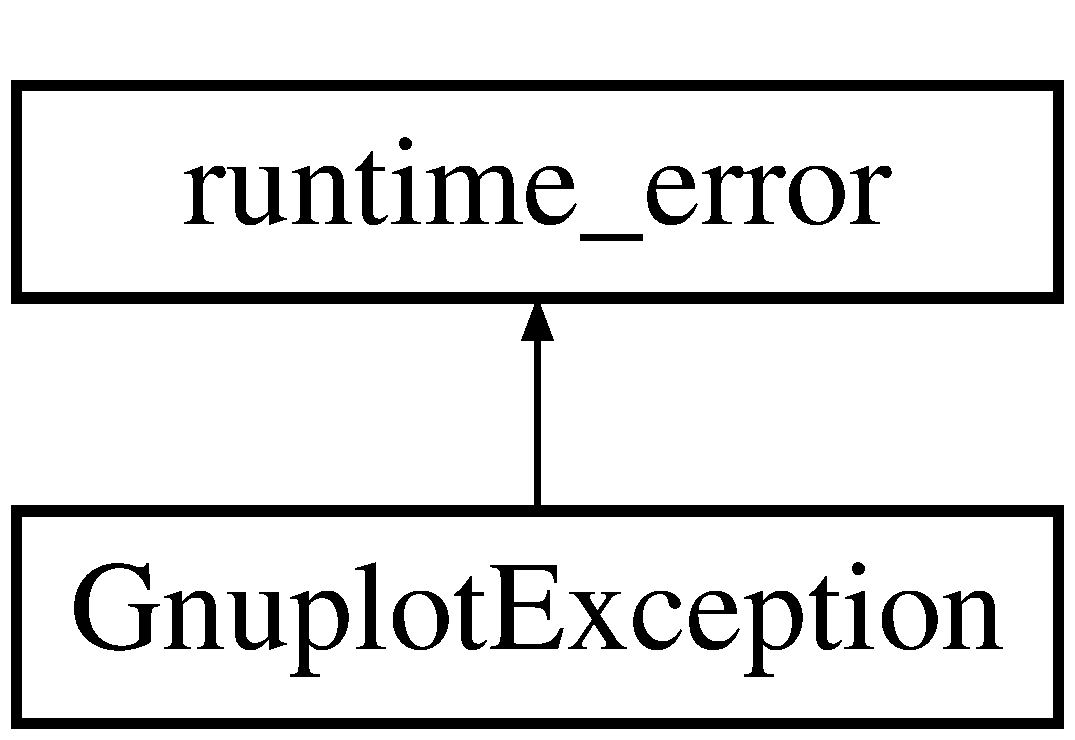
\includegraphics[height=2.000000cm]{class_gnuplot_exception}
\end{center}
\end{figure}
\subsection*{Public Member Functions}
\begin{DoxyCompactItemize}
\item 
\mbox{\hyperlink{class_gnuplot_exception_a81fc74a5c019556a4d0ba2a042a63448}{Gnuplot\+Exception}} (const string \&msg)
\end{DoxyCompactItemize}


\subsection{Detailed Description}


Definition at line 48 of file gnuplot\+\_\+i.\+hpp.



\subsection{Constructor \& Destructor Documentation}
\mbox{\Hypertarget{class_gnuplot_exception_a81fc74a5c019556a4d0ba2a042a63448}\label{class_gnuplot_exception_a81fc74a5c019556a4d0ba2a042a63448}} 
\index{Gnuplot\+Exception@{Gnuplot\+Exception}!Gnuplot\+Exception@{Gnuplot\+Exception}}
\index{Gnuplot\+Exception@{Gnuplot\+Exception}!Gnuplot\+Exception@{Gnuplot\+Exception}}
\subsubsection{\texorpdfstring{Gnuplot\+Exception()}{GnuplotException()}}
{\footnotesize\ttfamily Gnuplot\+Exception\+::\+Gnuplot\+Exception (\begin{DoxyParamCaption}\item[{const string \&}]{msg }\end{DoxyParamCaption})\hspace{0.3cm}{\ttfamily [inline]}}



Definition at line 51 of file gnuplot\+\_\+i.\+hpp.



The documentation for this class was generated from the following file\+:\begin{DoxyCompactItemize}
\item 
/\+Users/davidcleres/\+C\+Lion\+Projects/\+P\+C\+S\+C2017\+\_\+\+Group5/\mbox{\hyperlink{gnuplot__i_8hpp}{gnuplot\+\_\+i.\+hpp}}\end{DoxyCompactItemize}

\hypertarget{class_graph}{}\section{Graph Class Reference}
\label{class_graph}\index{Graph@{Graph}}


{\ttfamily \#include $<$Graph.\+h$>$}

\subsection*{Public Member Functions}
\begin{DoxyCompactItemize}
\item 
\mbox{\hyperlink{class_graph_ac2cc4f7971589f9674f4fbf3b7dc200c}{Graph}} (\mbox{\hyperlink{struct_data}{Data}} const \&data)
\begin{DoxyCompactList}\small\item\em Constructor of the class graph. \end{DoxyCompactList}\item 
void \mbox{\hyperlink{class_graph_af3560cb4e5eaa08c33e3de253a4e60a3}{make\+\_\+graph\+\_\+least\+\_\+square}} (size\+\_\+t const \&degree) const
\begin{DoxyCompactList}\small\item\em plots the graph for the least square regression \end{DoxyCompactList}\item 
void \mbox{\hyperlink{class_graph_a5fd01460d3981748a22269f9953d3486}{make\+\_\+graph\+\_\+lagrange}} () const
\begin{DoxyCompactList}\small\item\em plots the graph for the lagrange polynoma regression \end{DoxyCompactList}\item 
void \mbox{\hyperlink{class_graph_a00bb733092d1c97735b6fbc767a8cedf}{make\+\_\+graph\+\_\+piece\+\_\+wise\+\_\+least\+\_\+squares}} (size\+\_\+t const \&degree, int const \&intervalle) const
\begin{DoxyCompactList}\small\item\em Plots the graph for the least square regression. \end{DoxyCompactList}\item 
void \mbox{\hyperlink{class_graph_a4de7bd5074f188b470392920df1c7ada}{make\+\_\+graph\+\_\+piece\+\_\+wise\+\_\+lagrange}} (int const \&intervalle)
\begin{DoxyCompactList}\small\item\em Plots the graph for the lagrange regression. \end{DoxyCompactList}\item 
void \mbox{\hyperlink{class_graph_a5326be30b090c2ba956d0e0211895fcd}{make\+\_\+graph\+\_\+\+F\+FT}} (\mbox{\hyperlink{struct_data}{Data}} data\+\_\+original)
\begin{DoxyCompactList}\small\item\em Plots the graph for fourier approximation. \end{DoxyCompactList}\end{DoxyCompactItemize}


\subsection{Detailed Description}
(Note, this needs exactly one 

Definition at line 29 of file Graph.\+h.



\subsection{Constructor \& Destructor Documentation}
\mbox{\Hypertarget{class_graph_ac2cc4f7971589f9674f4fbf3b7dc200c}\label{class_graph_ac2cc4f7971589f9674f4fbf3b7dc200c}} 
\index{Graph@{Graph}!Graph@{Graph}}
\index{Graph@{Graph}!Graph@{Graph}}
\subsubsection{\texorpdfstring{Graph()}{Graph()}}
{\footnotesize\ttfamily Graph\+::\+Graph (\begin{DoxyParamCaption}\item[{\mbox{\hyperlink{struct_data}{Data}} const \&}]{data }\end{DoxyParamCaption})\hspace{0.3cm}{\ttfamily [explicit]}}



Constructor of the class graph. 


\begin{DoxyParams}{Parameters}
{\em data} & is a structure that contains the information about the X and Y axis \\
\hline
\end{DoxyParams}


Definition at line 10 of file Graph.\+cpp.



\subsection{Member Function Documentation}
\mbox{\Hypertarget{class_graph_a5326be30b090c2ba956d0e0211895fcd}\label{class_graph_a5326be30b090c2ba956d0e0211895fcd}} 
\index{Graph@{Graph}!make\+\_\+graph\+\_\+\+F\+FT@{make\+\_\+graph\+\_\+\+F\+FT}}
\index{make\+\_\+graph\+\_\+\+F\+FT@{make\+\_\+graph\+\_\+\+F\+FT}!Graph@{Graph}}
\subsubsection{\texorpdfstring{make\+\_\+graph\+\_\+\+F\+F\+T()}{make\_graph\_FFT()}}
{\footnotesize\ttfamily void Graph\+::make\+\_\+graph\+\_\+\+F\+FT (\begin{DoxyParamCaption}\item[{\mbox{\hyperlink{struct_data}{Data}}}]{data\+\_\+original }\end{DoxyParamCaption})}



Plots the graph for fourier approximation. 


\begin{DoxyParams}{Parameters}
{\em data\+\_\+original} & is the data as it is in the file \\
\hline
\end{DoxyParams}


Definition at line 114 of file Graph.\+cpp.

\mbox{\Hypertarget{class_graph_a5fd01460d3981748a22269f9953d3486}\label{class_graph_a5fd01460d3981748a22269f9953d3486}} 
\index{Graph@{Graph}!make\+\_\+graph\+\_\+lagrange@{make\+\_\+graph\+\_\+lagrange}}
\index{make\+\_\+graph\+\_\+lagrange@{make\+\_\+graph\+\_\+lagrange}!Graph@{Graph}}
\subsubsection{\texorpdfstring{make\+\_\+graph\+\_\+lagrange()}{make\_graph\_lagrange()}}
{\footnotesize\ttfamily void Graph\+::make\+\_\+graph\+\_\+lagrange (\begin{DoxyParamCaption}{ }\end{DoxyParamCaption}) const}



plots the graph for the lagrange polynoma regression 

Plot/// 

Definition at line 51 of file Graph.\+cpp.

\mbox{\Hypertarget{class_graph_af3560cb4e5eaa08c33e3de253a4e60a3}\label{class_graph_af3560cb4e5eaa08c33e3de253a4e60a3}} 
\index{Graph@{Graph}!make\+\_\+graph\+\_\+least\+\_\+square@{make\+\_\+graph\+\_\+least\+\_\+square}}
\index{make\+\_\+graph\+\_\+least\+\_\+square@{make\+\_\+graph\+\_\+least\+\_\+square}!Graph@{Graph}}
\subsubsection{\texorpdfstring{make\+\_\+graph\+\_\+least\+\_\+square()}{make\_graph\_least\_square()}}
{\footnotesize\ttfamily void Graph\+::make\+\_\+graph\+\_\+least\+\_\+square (\begin{DoxyParamCaption}\item[{size\+\_\+t const \&}]{degree }\end{DoxyParamCaption}) const}



plots the graph for the least square regression 


\begin{DoxyParams}{Parameters}
{\em degree} & is a positive integer that represents the degree of the fitted polynome \\
\hline
\end{DoxyParams}
Plot/// 

Definition at line 15 of file Graph.\+cpp.

\mbox{\Hypertarget{class_graph_a4de7bd5074f188b470392920df1c7ada}\label{class_graph_a4de7bd5074f188b470392920df1c7ada}} 
\index{Graph@{Graph}!make\+\_\+graph\+\_\+piece\+\_\+wise\+\_\+lagrange@{make\+\_\+graph\+\_\+piece\+\_\+wise\+\_\+lagrange}}
\index{make\+\_\+graph\+\_\+piece\+\_\+wise\+\_\+lagrange@{make\+\_\+graph\+\_\+piece\+\_\+wise\+\_\+lagrange}!Graph@{Graph}}
\subsubsection{\texorpdfstring{make\+\_\+graph\+\_\+piece\+\_\+wise\+\_\+lagrange()}{make\_graph\_piece\_wise\_lagrange()}}
{\footnotesize\ttfamily void Graph\+::make\+\_\+graph\+\_\+piece\+\_\+wise\+\_\+lagrange (\begin{DoxyParamCaption}\item[{int const \&}]{intervalle }\end{DoxyParamCaption})}



Plots the graph for the lagrange regression. 


\begin{DoxyParams}{Parameters}
{\em intervalle} & is the intervall for the the leat square method \\
\hline
\end{DoxyParams}


Definition at line 96 of file Graph.\+cpp.

\mbox{\Hypertarget{class_graph_a00bb733092d1c97735b6fbc767a8cedf}\label{class_graph_a00bb733092d1c97735b6fbc767a8cedf}} 
\index{Graph@{Graph}!make\+\_\+graph\+\_\+piece\+\_\+wise\+\_\+least\+\_\+squares@{make\+\_\+graph\+\_\+piece\+\_\+wise\+\_\+least\+\_\+squares}}
\index{make\+\_\+graph\+\_\+piece\+\_\+wise\+\_\+least\+\_\+squares@{make\+\_\+graph\+\_\+piece\+\_\+wise\+\_\+least\+\_\+squares}!Graph@{Graph}}
\subsubsection{\texorpdfstring{make\+\_\+graph\+\_\+piece\+\_\+wise\+\_\+least\+\_\+squares()}{make\_graph\_piece\_wise\_least\_squares()}}
{\footnotesize\ttfamily void Graph\+::make\+\_\+graph\+\_\+piece\+\_\+wise\+\_\+least\+\_\+squares (\begin{DoxyParamCaption}\item[{size\+\_\+t const \&}]{degree,  }\item[{int const \&}]{intervalle }\end{DoxyParamCaption}) const}



Plots the graph for the least square regression. 


\begin{DoxyParams}{Parameters}
{\em degree} & is a positive integer that represents the degree of the fitted polynome \\
\hline
{\em intervalle} & is the intervall for the the leat square method \\
\hline
\end{DoxyParams}
Plot/// 

Definition at line 76 of file Graph.\+cpp.



The documentation for this class was generated from the following files\+:\begin{DoxyCompactItemize}
\item 
/\+Users/davidcleres/\+C\+Lion\+Projects/\+P\+C\+S\+C2017\+\_\+\+Group5/\mbox{\hyperlink{_graph_8h}{Graph.\+h}}\item 
/\+Users/davidcleres/\+C\+Lion\+Projects/\+P\+C\+S\+C2017\+\_\+\+Group5/\mbox{\hyperlink{_graph_8cpp}{Graph.\+cpp}}\end{DoxyCompactItemize}

\hypertarget{class_lagrange}{}\section{Lagrange Class Reference}
\label{class_lagrange}\index{Lagrange@{Lagrange}}


This is redefinition of the virtual class to implement \mbox{\hyperlink{class_lagrange}{Lagrange}} functions

This is how we can calculate the approximation of the data using \mbox{\hyperlink{class_lagrange}{Lagrange}} Polynome.  




{\ttfamily \#include $<$Lagrange.\+h$>$}

\subsection*{Public Member Functions}
\begin{DoxyCompactItemize}
\item 
double \mbox{\hyperlink{class_lagrange_a9040a01112a83bbefb0f1bef1d7983bb}{solve}} (vector$<$ double $>$ const \&data\+\_\+x, vector$<$ double $>$ const \&data\+\_\+y, double xi)
\begin{DoxyCompactList}\small\item\em \mbox{\hyperlink{class_lagrange}{Lagrange}} return directly the point corresponding to the argument xi. \end{DoxyCompactList}\end{DoxyCompactItemize}


\subsection{Detailed Description}
This is redefinition of the virtual class to implement \mbox{\hyperlink{class_lagrange}{Lagrange}} functions

This is how we can calculate the approximation of the data using \mbox{\hyperlink{class_lagrange}{Lagrange}} Polynome. 

Definition at line 40 of file Lagrange.\+h.



\subsection{Member Function Documentation}
\mbox{\Hypertarget{class_lagrange_a9040a01112a83bbefb0f1bef1d7983bb}\label{class_lagrange_a9040a01112a83bbefb0f1bef1d7983bb}} 
\index{Lagrange@{Lagrange}!solve@{solve}}
\index{solve@{solve}!Lagrange@{Lagrange}}
\subsubsection{\texorpdfstring{solve()}{solve()}}
{\footnotesize\ttfamily double Lagrange\+::solve (\begin{DoxyParamCaption}\item[{vector$<$ double $>$ const \&}]{data\+\_\+x,  }\item[{vector$<$ double $>$ const \&}]{data\+\_\+y,  }\item[{double}]{xi }\end{DoxyParamCaption})}



\mbox{\hyperlink{class_lagrange}{Lagrange}} return directly the point corresponding to the argument xi. 

\mbox{\hyperlink{class_polynomial}{Polynomial}} approximation by the \mbox{\hyperlink{class_lagrange}{Lagrange}} algorithm.


\begin{DoxyParams}{Parameters}
{\em data\+\_\+x} & is a vector with the values read from the data.\+dat file \\
\hline
{\em data\+\_\+y} & is a vector with the values read from the data.\+dat file, if we have only real entries then you have to specify a vector with the same size as real but filled with zeros. \\
\hline
{\em xi} & \\
\hline
\end{DoxyParams}


Definition at line 9 of file Lagrange.\+cpp.



The documentation for this class was generated from the following files\+:\begin{DoxyCompactItemize}
\item 
/\+Users/davidcleres/\+C\+Lion\+Projects/\+P\+C\+S\+C2017\+\_\+\+Group5/\mbox{\hyperlink{_lagrange_8h}{Lagrange.\+h}}\item 
/\+Users/davidcleres/\+C\+Lion\+Projects/\+P\+C\+S\+C2017\+\_\+\+Group5/\mbox{\hyperlink{_lagrange_8cpp}{Lagrange.\+cpp}}\end{DoxyCompactItemize}

\hypertarget{class_piece_wise___continue___polynomial}{}\section{Piece\+Wise\+\_\+\+Continue\+\_\+\+Polynomial Class Reference}
\label{class_piece_wise___continue___polynomial}\index{Piece\+Wise\+\_\+\+Continue\+\_\+\+Polynomial@{Piece\+Wise\+\_\+\+Continue\+\_\+\+Polynomial}}


{\ttfamily \#include $<$Piece\+Wise\+\_\+\+Continue\+\_\+\+Polynomial.\+h$>$}

Inheritance diagram for Piece\+Wise\+\_\+\+Continue\+\_\+\+Polynomial\+:\begin{figure}[H]
\begin{center}
\leavevmode
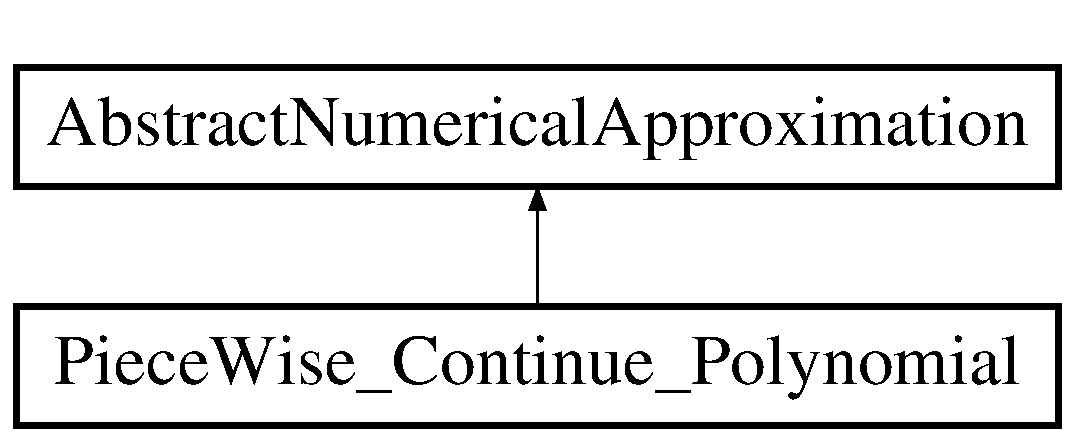
\includegraphics[height=2.000000cm]{class_piece_wise___continue___polynomial}
\end{center}
\end{figure}
\subsection*{Public Member Functions}
\begin{DoxyCompactItemize}
\item 
vector$<$ double $>$ \mbox{\hyperlink{class_piece_wise___continue___polynomial_a78a6e7994a1a007806da7d0cc8047413}{solve}} (\mbox{\hyperlink{struct_data}{Data}} data, int degree, int Intervale, vector$<$ double $>$x\+\_\+plot)
\begin{DoxyCompactList}\small\item\em Piece-\/wise polynomial approximation with continuous derivative using polynoms. \end{DoxyCompactList}\end{DoxyCompactItemize}


\subsection{Detailed Description}


Definition at line 15 of file Piece\+Wise\+\_\+\+Continue\+\_\+\+Polynomial.\+h.



\subsection{Member Function Documentation}
\mbox{\Hypertarget{class_piece_wise___continue___polynomial_a78a6e7994a1a007806da7d0cc8047413}\label{class_piece_wise___continue___polynomial_a78a6e7994a1a007806da7d0cc8047413}} 
\index{Piece\+Wise\+\_\+\+Continue\+\_\+\+Polynomial@{Piece\+Wise\+\_\+\+Continue\+\_\+\+Polynomial}!solve@{solve}}
\index{solve@{solve}!Piece\+Wise\+\_\+\+Continue\+\_\+\+Polynomial@{Piece\+Wise\+\_\+\+Continue\+\_\+\+Polynomial}}
\subsubsection{\texorpdfstring{solve()}{solve()}}
{\footnotesize\ttfamily vector$<$ double $>$ Piece\+Wise\+\_\+\+Continue\+\_\+\+Polynomial\+::solve (\begin{DoxyParamCaption}\item[{\mbox{\hyperlink{struct_data}{Data}}}]{data,  }\item[{int}]{degree,  }\item[{int}]{Intervale,  }\item[{vector$<$ double $>$}]{x\+\_\+plot }\end{DoxyParamCaption})}



Piece-\/wise polynomial approximation with continuous derivative using polynoms. 



Definition at line 17 of file Piece\+Wise\+\_\+\+Continue\+\_\+\+Polynomial.\+cpp.



The documentation for this class was generated from the following files\+:\begin{DoxyCompactItemize}
\item 
/\+Users/davidcleres/\+C\+Lion\+Projects/\+P\+C\+S\+C2017\+\_\+\+Group5/\mbox{\hyperlink{_piece_wise___continue___polynomial_8h}{Piece\+Wise\+\_\+\+Continue\+\_\+\+Polynomial.\+h}}\item 
/\+Users/davidcleres/\+C\+Lion\+Projects/\+P\+C\+S\+C2017\+\_\+\+Group5/\mbox{\hyperlink{_piece_wise___continue___polynomial_8cpp}{Piece\+Wise\+\_\+\+Continue\+\_\+\+Polynomial.\+cpp}}\end{DoxyCompactItemize}

\hypertarget{class_point}{}\section{Point Class Reference}
\label{class_point}\index{Point@{Point}}


{\ttfamily \#include $<$Point.\+h$>$}

\subsection*{Public Member Functions}
\begin{DoxyCompactItemize}
\item 
\mbox{\hyperlink{class_point_a44d490126797f9e88de376fb6814b089}{Point}} (size\+\_\+t const \&taille)
\begin{DoxyCompactList}\small\item\em Constructor. \end{DoxyCompactList}\item 
\mbox{\hyperlink{class_point_a64da1fdafc9131972f1458ef9bd5de30}{Point}} (vector$<$ double $>$ const \&x, vector$<$ double $>$ const \&y)
\begin{DoxyCompactList}\small\item\em Constructor. \end{DoxyCompactList}\item 
vector$<$ double $>$ \mbox{\hyperlink{class_point_a0badc8959ee9db08740cf22abcb8d8db}{get\+\_\+x}} () const
\begin{DoxyCompactList}\small\item\em returns the value of mx \end{DoxyCompactList}\item 
vector$<$ double $>$ \mbox{\hyperlink{class_point_a5d9ab69bfb09db813d543a8cd2fb24c7}{get\+\_\+y}} () const
\begin{DoxyCompactList}\small\item\em returns the value of my \end{DoxyCompactList}\item 
void \mbox{\hyperlink{class_point_a7a9b270860e9198583176ad5c42f9187}{set\+\_\+x}} (size\+\_\+t const \&index, double const \&value)
\begin{DoxyCompactList}\small\item\em setter for x \end{DoxyCompactList}\item 
void \mbox{\hyperlink{class_point_a40f61acc21fc1416c2cc1034ee2a928a}{set\+\_\+y}} (size\+\_\+t const \&index, double const \&value)
\begin{DoxyCompactList}\small\item\em setter for y \end{DoxyCompactList}\end{DoxyCompactItemize}


\subsection{Detailed Description}
(Note, this needs exactly one 

Definition at line 31 of file Point.\+h.



\subsection{Constructor \& Destructor Documentation}
\mbox{\Hypertarget{class_point_a44d490126797f9e88de376fb6814b089}\label{class_point_a44d490126797f9e88de376fb6814b089}} 
\index{Point@{Point}!Point@{Point}}
\index{Point@{Point}!Point@{Point}}
\subsubsection{\texorpdfstring{Point()}{Point()}\hspace{0.1cm}{\footnotesize\ttfamily [1/2]}}
{\footnotesize\ttfamily Point\+::\+Point (\begin{DoxyParamCaption}\item[{size\+\_\+t const \&}]{taille }\end{DoxyParamCaption})\hspace{0.3cm}{\ttfamily [explicit]}}



Constructor. 


\begin{DoxyParams}{Parameters}
{\em taille} & is the size of the vector \\
\hline
\end{DoxyParams}


Definition at line 9 of file Point.\+cpp.

\mbox{\Hypertarget{class_point_a64da1fdafc9131972f1458ef9bd5de30}\label{class_point_a64da1fdafc9131972f1458ef9bd5de30}} 
\index{Point@{Point}!Point@{Point}}
\index{Point@{Point}!Point@{Point}}
\subsubsection{\texorpdfstring{Point()}{Point()}\hspace{0.1cm}{\footnotesize\ttfamily [2/2]}}
{\footnotesize\ttfamily Point\+::\+Point (\begin{DoxyParamCaption}\item[{vector$<$ double $>$ const \&}]{x,  }\item[{vector$<$ double $>$ const \&}]{y }\end{DoxyParamCaption})}



Constructor. 


\begin{DoxyParams}{Parameters}
{\em x} & is a vector with the values of approximate (x-\/axis) \\
\hline
{\em y} & is a vector with the values of approximate (y-\/axis) \\
\hline
\end{DoxyParams}


Definition at line 14 of file Point.\+cpp.



\subsection{Member Function Documentation}
\mbox{\Hypertarget{class_point_a0badc8959ee9db08740cf22abcb8d8db}\label{class_point_a0badc8959ee9db08740cf22abcb8d8db}} 
\index{Point@{Point}!get\+\_\+x@{get\+\_\+x}}
\index{get\+\_\+x@{get\+\_\+x}!Point@{Point}}
\subsubsection{\texorpdfstring{get\+\_\+x()}{get\_x()}}
{\footnotesize\ttfamily vector$<$ double $>$ Point\+::get\+\_\+x (\begin{DoxyParamCaption}{ }\end{DoxyParamCaption}) const}



returns the value of mx 



Definition at line 21 of file Point.\+cpp.

\mbox{\Hypertarget{class_point_a5d9ab69bfb09db813d543a8cd2fb24c7}\label{class_point_a5d9ab69bfb09db813d543a8cd2fb24c7}} 
\index{Point@{Point}!get\+\_\+y@{get\+\_\+y}}
\index{get\+\_\+y@{get\+\_\+y}!Point@{Point}}
\subsubsection{\texorpdfstring{get\+\_\+y()}{get\_y()}}
{\footnotesize\ttfamily vector$<$ double $>$ Point\+::get\+\_\+y (\begin{DoxyParamCaption}{ }\end{DoxyParamCaption}) const}



returns the value of my 



Definition at line 25 of file Point.\+cpp.

\mbox{\Hypertarget{class_point_a7a9b270860e9198583176ad5c42f9187}\label{class_point_a7a9b270860e9198583176ad5c42f9187}} 
\index{Point@{Point}!set\+\_\+x@{set\+\_\+x}}
\index{set\+\_\+x@{set\+\_\+x}!Point@{Point}}
\subsubsection{\texorpdfstring{set\+\_\+x()}{set\_x()}}
{\footnotesize\ttfamily void Point\+::set\+\_\+x (\begin{DoxyParamCaption}\item[{size\+\_\+t const \&}]{index,  }\item[{double const \&}]{value }\end{DoxyParamCaption})}



setter for x 


\begin{DoxyParams}{Parameters}
{\em index} & \\
\hline
{\em value} & \\
\hline
\end{DoxyParams}


Definition at line 30 of file Point.\+cpp.

\mbox{\Hypertarget{class_point_a40f61acc21fc1416c2cc1034ee2a928a}\label{class_point_a40f61acc21fc1416c2cc1034ee2a928a}} 
\index{Point@{Point}!set\+\_\+y@{set\+\_\+y}}
\index{set\+\_\+y@{set\+\_\+y}!Point@{Point}}
\subsubsection{\texorpdfstring{set\+\_\+y()}{set\_y()}}
{\footnotesize\ttfamily void Point\+::set\+\_\+y (\begin{DoxyParamCaption}\item[{size\+\_\+t const \&}]{index,  }\item[{double const \&}]{value }\end{DoxyParamCaption})}



setter for y 


\begin{DoxyParams}{Parameters}
{\em index} & \\
\hline
{\em value} & \\
\hline
\end{DoxyParams}


Definition at line 34 of file Point.\+cpp.



The documentation for this class was generated from the following files\+:\begin{DoxyCompactItemize}
\item 
/\+Users/davidcleres/\+C\+Lion\+Projects/\+P\+C\+S\+C2017\+\_\+\+Group5/\mbox{\hyperlink{_point_8h}{Point.\+h}}\item 
/\+Users/davidcleres/\+C\+Lion\+Projects/\+P\+C\+S\+C2017\+\_\+\+Group5/\mbox{\hyperlink{_point_8cpp}{Point.\+cpp}}\end{DoxyCompactItemize}

\hypertarget{structpoint__t}{}\section{point\+\_\+t Struct Reference}
\label{structpoint__t}\index{point\+\_\+t@{point\+\_\+t}}


{\ttfamily \#include $<$read\+File.\+h$>$}

\subsection*{Public Attributes}
\begin{DoxyCompactItemize}
\item 
double \mbox{\hyperlink{structpoint__t_acf7556ca44360564040f5c86257b55b1}{x}}
\item 
double \mbox{\hyperlink{structpoint__t_a8590af4986d0e4ef2b6756946f80438c}{y}}
\end{DoxyCompactItemize}


\subsection{Detailed Description}


Definition at line 38 of file read\+File.\+h.



\subsection{Member Data Documentation}
\mbox{\Hypertarget{structpoint__t_acf7556ca44360564040f5c86257b55b1}\label{structpoint__t_acf7556ca44360564040f5c86257b55b1}} 
\index{point\+\_\+t@{point\+\_\+t}!x@{x}}
\index{x@{x}!point\+\_\+t@{point\+\_\+t}}
\subsubsection{\texorpdfstring{x}{x}}
{\footnotesize\ttfamily double point\+\_\+t\+::x}



Definition at line 39 of file read\+File.\+h.

\mbox{\Hypertarget{structpoint__t_a8590af4986d0e4ef2b6756946f80438c}\label{structpoint__t_a8590af4986d0e4ef2b6756946f80438c}} 
\index{point\+\_\+t@{point\+\_\+t}!y@{y}}
\index{y@{y}!point\+\_\+t@{point\+\_\+t}}
\subsubsection{\texorpdfstring{y}{y}}
{\footnotesize\ttfamily double point\+\_\+t\+::y}



Definition at line 40 of file read\+File.\+h.



The documentation for this struct was generated from the following file\+:\begin{DoxyCompactItemize}
\item 
/\+Users/davidcleres/\+C\+Lion\+Projects/\+P\+C\+S\+C2017\+\_\+\+Group5/\mbox{\hyperlink{read_file_8h}{read\+File.\+h}}\end{DoxyCompactItemize}

\hypertarget{class_polynomial}{}\section{Polynomial Class Reference}
\label{class_polynomial}\index{Polynomial@{Polynomial}}


{\ttfamily \#include $<$Polynomial.\+h$>$}

\subsection*{Public Member Functions}
\begin{DoxyCompactItemize}
\item 
vector$<$ double $>$ \mbox{\hyperlink{class_polynomial_ae67730df0a2e45a87c9cb244fe03ad6b}{solve}} (vector$<$ double $>$ const \&data, vector$<$ double $>$ const \&data\+\_\+y, size\+\_\+t const \&degree)
\begin{DoxyCompactList}\small\item\em solve the linear equation \end{DoxyCompactList}\end{DoxyCompactItemize}


\subsection{Detailed Description}
(Note, this needs exactly one 

Definition at line 32 of file Polynomial.\+h.



\subsection{Member Function Documentation}
\mbox{\Hypertarget{class_polynomial_ae67730df0a2e45a87c9cb244fe03ad6b}\label{class_polynomial_ae67730df0a2e45a87c9cb244fe03ad6b}} 
\index{Polynomial@{Polynomial}!solve@{solve}}
\index{solve@{solve}!Polynomial@{Polynomial}}
\subsubsection{\texorpdfstring{solve()}{solve()}}
{\footnotesize\ttfamily vector$<$ double $>$ Polynomial\+::solve (\begin{DoxyParamCaption}\item[{vector$<$ double $>$ const \&}]{data,  }\item[{vector$<$ double $>$ const \&}]{data\+\_\+y,  }\item[{size\+\_\+t const \&}]{degree }\end{DoxyParamCaption})}



solve the linear equation 

\mbox{\hyperlink{class_polynomial}{Polynomial}} approximation of the given points using a single polynome.


\begin{DoxyParams}{Parameters}
{\em data} & is a vector with the values of approximate (x-\/axis) \\
\hline
{\em degree} & is the degree of the polynome \\
\hline
{\em data\+\_\+y} & is a vector with the values of approximate (y-\/axis) \\
\hline
\end{DoxyParams}


Definition at line 12 of file Polynomial.\+cpp.



The documentation for this class was generated from the following files\+:\begin{DoxyCompactItemize}
\item 
/\+Users/davidcleres/\+C\+Lion\+Projects/\+P\+C\+S\+C2017\+\_\+\+Group5/\mbox{\hyperlink{_polynomial_8h}{Polynomial.\+h}}\item 
/\+Users/davidcleres/\+C\+Lion\+Projects/\+P\+C\+S\+C2017\+\_\+\+Group5/\mbox{\hyperlink{_polynomial_8cpp}{Polynomial.\+cpp}}\end{DoxyCompactItemize}

\hypertarget{class_read_file}{}\section{Read\+File Class Reference}
\label{class_read_file}\index{Read\+File@{Read\+File}}


{\ttfamily \#include $<$read\+File.\+h$>$}

\subsection*{Public Member Functions}
\begin{DoxyCompactItemize}
\item 
\mbox{\hyperlink{class_read_file_ae297f0539380fc9b703a1bceda2ce820}{Read\+File}} (std\+::string const \&filename)
\item 
void \mbox{\hyperlink{class_read_file_a232df426223b84e4dbb3f964ee4c3177}{load\+From\+File}} (\mbox{\hyperlink{struct_data}{Data}} \&data)
\item 
std\+::string \mbox{\hyperlink{class_read_file_a9835264c9ec95cfdbc1349573402fc01}{get\+Filename}} ()
\item 
void \mbox{\hyperlink{class_read_file_a5efc41b900510ae038dafc23a2563300}{show}} (\mbox{\hyperlink{struct_data}{Data}} const \&data)
\item 
void \mbox{\hyperlink{class_read_file_ac11779a3630a2c1d62ab4566abb4034a}{write\+File}} (\mbox{\hyperlink{struct_data}{Data}} const \&data)
\end{DoxyCompactItemize}


\subsection{Detailed Description}


Definition at line 32 of file read\+File.\+h.



\subsection{Constructor \& Destructor Documentation}
\mbox{\Hypertarget{class_read_file_ae297f0539380fc9b703a1bceda2ce820}\label{class_read_file_ae297f0539380fc9b703a1bceda2ce820}} 
\index{Read\+File@{Read\+File}!Read\+File@{Read\+File}}
\index{Read\+File@{Read\+File}!Read\+File@{Read\+File}}
\subsubsection{\texorpdfstring{Read\+File()}{ReadFile()}}
{\footnotesize\ttfamily Read\+File\+::\+Read\+File (\begin{DoxyParamCaption}\item[{std\+::string const \&}]{filename }\end{DoxyParamCaption})\hspace{0.3cm}{\ttfamily [explicit]}}







Definition at line 54 of file read\+File.\+cpp.



\subsection{Member Function Documentation}
\mbox{\Hypertarget{class_read_file_a9835264c9ec95cfdbc1349573402fc01}\label{class_read_file_a9835264c9ec95cfdbc1349573402fc01}} 
\index{Read\+File@{Read\+File}!get\+Filename@{get\+Filename}}
\index{get\+Filename@{get\+Filename}!Read\+File@{Read\+File}}
\subsubsection{\texorpdfstring{get\+Filename()}{getFilename()}}
{\footnotesize\ttfamily std\+::string Read\+File\+::get\+Filename (\begin{DoxyParamCaption}{ }\end{DoxyParamCaption})}







Definition at line 58 of file read\+File.\+cpp.

\mbox{\Hypertarget{class_read_file_a232df426223b84e4dbb3f964ee4c3177}\label{class_read_file_a232df426223b84e4dbb3f964ee4c3177}} 
\index{Read\+File@{Read\+File}!load\+From\+File@{load\+From\+File}}
\index{load\+From\+File@{load\+From\+File}!Read\+File@{Read\+File}}
\subsubsection{\texorpdfstring{load\+From\+File()}{loadFromFile()}}
{\footnotesize\ttfamily void Read\+File\+::load\+From\+File (\begin{DoxyParamCaption}\item[{\mbox{\hyperlink{struct_data}{Data}} \&}]{data }\end{DoxyParamCaption})}







Definition at line 13 of file read\+File.\+cpp.

\mbox{\Hypertarget{class_read_file_a5efc41b900510ae038dafc23a2563300}\label{class_read_file_a5efc41b900510ae038dafc23a2563300}} 
\index{Read\+File@{Read\+File}!show@{show}}
\index{show@{show}!Read\+File@{Read\+File}}
\subsubsection{\texorpdfstring{show()}{show()}}
{\footnotesize\ttfamily void Read\+File\+::show (\begin{DoxyParamCaption}\item[{\mbox{\hyperlink{struct_data}{Data}} const \&}]{data }\end{DoxyParamCaption})}







Definition at line 62 of file read\+File.\+cpp.

\mbox{\Hypertarget{class_read_file_ac11779a3630a2c1d62ab4566abb4034a}\label{class_read_file_ac11779a3630a2c1d62ab4566abb4034a}} 
\index{Read\+File@{Read\+File}!write\+File@{write\+File}}
\index{write\+File@{write\+File}!Read\+File@{Read\+File}}
\subsubsection{\texorpdfstring{write\+File()}{writeFile()}}
{\footnotesize\ttfamily void Read\+File\+::write\+File (\begin{DoxyParamCaption}\item[{\mbox{\hyperlink{struct_data}{Data}} const \&}]{data }\end{DoxyParamCaption})}







Definition at line 69 of file read\+File.\+cpp.



The documentation for this class was generated from the following files\+:\begin{DoxyCompactItemize}
\item 
/\+Users/davidcleres/\+C\+Lion\+Projects/\+P\+C\+S\+C2017\+\_\+\+Group5/\mbox{\hyperlink{read_file_8h}{read\+File.\+h}}\item 
/\+Users/davidcleres/\+C\+Lion\+Projects/\+P\+C\+S\+C2017\+\_\+\+Group5/\mbox{\hyperlink{read_file_8cpp}{read\+File.\+cpp}}\end{DoxyCompactItemize}

\hypertarget{class_reafile}{}\section{Reafile Class Reference}
\label{class_reafile}\index{Reafile@{Reafile}}


This is a simple positions accessor.  




{\ttfamily \#include $<$read\+File.\+h$>$}



\subsection{Detailed Description}
This is a simple positions accessor. 

The documentation for this class was generated from the following file\+:\begin{DoxyCompactItemize}
\item 
/\+Users/davidcleres/\+C\+Lion\+Projects/\+P\+C\+S\+C2017\+\_\+\+Group5/\mbox{\hyperlink{read_file_8h}{read\+File.\+h}}\end{DoxyCompactItemize}

\chapter{File Documentation}
\hypertarget{_c_make_c_compiler_id_8c}{}\section{/\+Users/davidcleres/\+C\+Lion\+Projects/\+P\+C\+S\+C2017\+\_\+\+Group5/cmake-\/build-\/debug/\+C\+Make\+Files/3.8.2/\+Compiler\+Id\+C/\+C\+Make\+C\+Compiler\+Id.c File Reference}
\label{_c_make_c_compiler_id_8c}\index{/\+Users/davidcleres/\+C\+Lion\+Projects/\+P\+C\+S\+C2017\+\_\+\+Group5/cmake-\/build-\/debug/\+C\+Make\+Files/3.\+8.\+2/\+Compiler\+Id\+C/\+C\+Make\+C\+Compiler\+Id.\+c@{/\+Users/davidcleres/\+C\+Lion\+Projects/\+P\+C\+S\+C2017\+\_\+\+Group5/cmake-\/build-\/debug/\+C\+Make\+Files/3.\+8.\+2/\+Compiler\+Id\+C/\+C\+Make\+C\+Compiler\+Id.\+c}}
\subsection*{Macros}
\begin{DoxyCompactItemize}
\item 
\#define \mbox{\hyperlink{_c_make_c_compiler_id_8c_a81dee0709ded976b2e0319239f72d174}{C\+O\+M\+P\+I\+L\+E\+R\+\_\+\+ID}}~\char`\"{}\char`\"{}
\item 
\#define \mbox{\hyperlink{_c_make_c_compiler_id_8c_a2ae9b72bb13abaabfcf2ee0ba7d3fa1d}{S\+T\+R\+I\+N\+G\+I\+F\+Y\+\_\+\+H\+E\+L\+P\+ER}}(X)~\#X
\item 
\#define \mbox{\hyperlink{_c_make_c_compiler_id_8c_a43e1cad902b6477bec893cb6430bd6c8}{S\+T\+R\+I\+N\+G\+I\+FY}}(X)~\mbox{\hyperlink{_c_make_c_x_x_compiler_id_8cpp_a2ae9b72bb13abaabfcf2ee0ba7d3fa1d}{S\+T\+R\+I\+N\+G\+I\+F\+Y\+\_\+\+H\+E\+L\+P\+ER}}(X)
\item 
\#define \mbox{\hyperlink{_c_make_c_compiler_id_8c_adbc5372f40838899018fadbc89bd588b}{P\+L\+A\+T\+F\+O\+R\+M\+\_\+\+ID}}
\item 
\#define \mbox{\hyperlink{_c_make_c_compiler_id_8c_aba35d0d200deaeb06aee95ca297acb28}{A\+R\+C\+H\+I\+T\+E\+C\+T\+U\+R\+E\+\_\+\+ID}}
\item 
\#define \mbox{\hyperlink{_c_make_c_compiler_id_8c_ad1280362da42492bbc11aa78cbf776ad}{D\+EC}}(n)
\item 
\#define \mbox{\hyperlink{_c_make_c_compiler_id_8c_a46d5d95daa1bef867bd0179594310ed5}{H\+EX}}(n)
\item 
\#define \mbox{\hyperlink{_c_make_c_compiler_id_8c_a07f8e5783674099cd7f5110e22a78cdb}{C\+\_\+\+D\+I\+A\+L\+E\+CT}}
\end{DoxyCompactItemize}
\subsection*{Functions}
\begin{DoxyCompactItemize}
\item 
int \mbox{\hyperlink{_c_make_c_compiler_id_8c_a0ddf1224851353fc92bfbff6f499fa97}{main}} (int argc, char $\ast$argv\mbox{[}$\,$\mbox{]})
\end{DoxyCompactItemize}
\subsection*{Variables}
\begin{DoxyCompactItemize}
\item 
char const  $\ast$ \mbox{\hyperlink{_c_make_c_compiler_id_8c_a4b0efeb7a5d59313986b3a0390f050f6}{info\+\_\+compiler}} = \char`\"{}I\+N\+FO\char`\"{} \char`\"{}\+:\char`\"{} \char`\"{}compiler\mbox{[}\char`\"{} C\+O\+M\+P\+I\+L\+E\+R\+\_\+\+ID \char`\"{}\mbox{]}\char`\"{}
\item 
char const  $\ast$ \mbox{\hyperlink{_c_make_c_compiler_id_8c_a2321403dee54ee23f0c2fa849c60f7d4}{info\+\_\+platform}} = \char`\"{}I\+N\+FO\char`\"{} \char`\"{}\+:\char`\"{} \char`\"{}platform\mbox{[}\char`\"{} P\+L\+A\+T\+F\+O\+R\+M\+\_\+\+ID \char`\"{}\mbox{]}\char`\"{}
\item 
char const  $\ast$ \mbox{\hyperlink{_c_make_c_compiler_id_8c_a59647e99d304ed33b15cb284c27ed391}{info\+\_\+arch}} = \char`\"{}I\+N\+FO\char`\"{} \char`\"{}\+:\char`\"{} \char`\"{}arch\mbox{[}\char`\"{} A\+R\+C\+H\+I\+T\+E\+C\+T\+U\+R\+E\+\_\+\+ID \char`\"{}\mbox{]}\char`\"{}
\item 
const char $\ast$ \mbox{\hyperlink{_c_make_c_compiler_id_8c_a1ce162bad2fe6966ac8b33cc19e120b8}{info\+\_\+language\+\_\+dialect\+\_\+default}}
\end{DoxyCompactItemize}


\subsection{Macro Definition Documentation}
\mbox{\Hypertarget{_c_make_c_compiler_id_8c_aba35d0d200deaeb06aee95ca297acb28}\label{_c_make_c_compiler_id_8c_aba35d0d200deaeb06aee95ca297acb28}} 
\index{C\+Make\+C\+Compiler\+Id.\+c@{C\+Make\+C\+Compiler\+Id.\+c}!A\+R\+C\+H\+I\+T\+E\+C\+T\+U\+R\+E\+\_\+\+ID@{A\+R\+C\+H\+I\+T\+E\+C\+T\+U\+R\+E\+\_\+\+ID}}
\index{A\+R\+C\+H\+I\+T\+E\+C\+T\+U\+R\+E\+\_\+\+ID@{A\+R\+C\+H\+I\+T\+E\+C\+T\+U\+R\+E\+\_\+\+ID}!C\+Make\+C\+Compiler\+Id.\+c@{C\+Make\+C\+Compiler\+Id.\+c}}
\subsubsection{\texorpdfstring{A\+R\+C\+H\+I\+T\+E\+C\+T\+U\+R\+E\+\_\+\+ID}{ARCHITECTURE\_ID}}
{\footnotesize\ttfamily \#define A\+R\+C\+H\+I\+T\+E\+C\+T\+U\+R\+E\+\_\+\+ID}



Definition at line 449 of file C\+Make\+C\+Compiler\+Id.\+c.

\mbox{\Hypertarget{_c_make_c_compiler_id_8c_a07f8e5783674099cd7f5110e22a78cdb}\label{_c_make_c_compiler_id_8c_a07f8e5783674099cd7f5110e22a78cdb}} 
\index{C\+Make\+C\+Compiler\+Id.\+c@{C\+Make\+C\+Compiler\+Id.\+c}!C\+\_\+\+D\+I\+A\+L\+E\+CT@{C\+\_\+\+D\+I\+A\+L\+E\+CT}}
\index{C\+\_\+\+D\+I\+A\+L\+E\+CT@{C\+\_\+\+D\+I\+A\+L\+E\+CT}!C\+Make\+C\+Compiler\+Id.\+c@{C\+Make\+C\+Compiler\+Id.\+c}}
\subsubsection{\texorpdfstring{C\+\_\+\+D\+I\+A\+L\+E\+CT}{C\_DIALECT}}
{\footnotesize\ttfamily \#define C\+\_\+\+D\+I\+A\+L\+E\+CT}



Definition at line 524 of file C\+Make\+C\+Compiler\+Id.\+c.

\mbox{\Hypertarget{_c_make_c_compiler_id_8c_a81dee0709ded976b2e0319239f72d174}\label{_c_make_c_compiler_id_8c_a81dee0709ded976b2e0319239f72d174}} 
\index{C\+Make\+C\+Compiler\+Id.\+c@{C\+Make\+C\+Compiler\+Id.\+c}!C\+O\+M\+P\+I\+L\+E\+R\+\_\+\+ID@{C\+O\+M\+P\+I\+L\+E\+R\+\_\+\+ID}}
\index{C\+O\+M\+P\+I\+L\+E\+R\+\_\+\+ID@{C\+O\+M\+P\+I\+L\+E\+R\+\_\+\+ID}!C\+Make\+C\+Compiler\+Id.\+c@{C\+Make\+C\+Compiler\+Id.\+c}}
\subsubsection{\texorpdfstring{C\+O\+M\+P\+I\+L\+E\+R\+\_\+\+ID}{COMPILER\_ID}}
{\footnotesize\ttfamily \#define C\+O\+M\+P\+I\+L\+E\+R\+\_\+\+ID~\char`\"{}\char`\"{}}



Definition at line 282 of file C\+Make\+C\+Compiler\+Id.\+c.

\mbox{\Hypertarget{_c_make_c_compiler_id_8c_ad1280362da42492bbc11aa78cbf776ad}\label{_c_make_c_compiler_id_8c_ad1280362da42492bbc11aa78cbf776ad}} 
\index{C\+Make\+C\+Compiler\+Id.\+c@{C\+Make\+C\+Compiler\+Id.\+c}!D\+EC@{D\+EC}}
\index{D\+EC@{D\+EC}!C\+Make\+C\+Compiler\+Id.\+c@{C\+Make\+C\+Compiler\+Id.\+c}}
\subsubsection{\texorpdfstring{D\+EC}{DEC}}
{\footnotesize\ttfamily \#define D\+EC(\begin{DoxyParamCaption}\item[{}]{n }\end{DoxyParamCaption})}

{\bfseries Value\+:}
\begin{DoxyCode}
(\textcolor{charliteral}{'0'} + (((n) / 10000000)%10)), \(\backslash\)
  (\textcolor{charliteral}{'0'} + (((n) / 1000000)%10)),  \(\backslash\)
  (\textcolor{charliteral}{'0'} + (((n) / 100000)%10)),   \(\backslash\)
  (\textcolor{charliteral}{'0'} + (((n) / 10000)%10)),    \(\backslash\)
  (\textcolor{charliteral}{'0'} + (((n) / 1000)%10)),     \(\backslash\)
  (\textcolor{charliteral}{'0'} + (((n) / 100)%10)),      \(\backslash\)
  (\textcolor{charliteral}{'0'} + (((n) / 10)%10)),       \(\backslash\)
  (\textcolor{charliteral}{'0'} +  ((n) % 10))
\end{DoxyCode}


Definition at line 453 of file C\+Make\+C\+Compiler\+Id.\+c.

\mbox{\Hypertarget{_c_make_c_compiler_id_8c_a46d5d95daa1bef867bd0179594310ed5}\label{_c_make_c_compiler_id_8c_a46d5d95daa1bef867bd0179594310ed5}} 
\index{C\+Make\+C\+Compiler\+Id.\+c@{C\+Make\+C\+Compiler\+Id.\+c}!H\+EX@{H\+EX}}
\index{H\+EX@{H\+EX}!C\+Make\+C\+Compiler\+Id.\+c@{C\+Make\+C\+Compiler\+Id.\+c}}
\subsubsection{\texorpdfstring{H\+EX}{HEX}}
{\footnotesize\ttfamily \#define H\+EX(\begin{DoxyParamCaption}\item[{}]{n }\end{DoxyParamCaption})}

{\bfseries Value\+:}
\begin{DoxyCode}
(\textcolor{charliteral}{'0'} + ((n)>>28 & 0xF)), \(\backslash\)
  (\textcolor{charliteral}{'0'} + ((n)>>24 & 0xF)), \(\backslash\)
  (\textcolor{charliteral}{'0'} + ((n)>>20 & 0xF)), \(\backslash\)
  (\textcolor{charliteral}{'0'} + ((n)>>16 & 0xF)), \(\backslash\)
  (\textcolor{charliteral}{'0'} + ((n)>>12 & 0xF)), \(\backslash\)
  (\textcolor{charliteral}{'0'} + ((n)>>8  & 0xF)), \(\backslash\)
  (\textcolor{charliteral}{'0'} + ((n)>>4  & 0xF)), \(\backslash\)
  (\textcolor{charliteral}{'0'} + ((n)     & 0xF))
\end{DoxyCode}


Definition at line 464 of file C\+Make\+C\+Compiler\+Id.\+c.

\mbox{\Hypertarget{_c_make_c_compiler_id_8c_adbc5372f40838899018fadbc89bd588b}\label{_c_make_c_compiler_id_8c_adbc5372f40838899018fadbc89bd588b}} 
\index{C\+Make\+C\+Compiler\+Id.\+c@{C\+Make\+C\+Compiler\+Id.\+c}!P\+L\+A\+T\+F\+O\+R\+M\+\_\+\+ID@{P\+L\+A\+T\+F\+O\+R\+M\+\_\+\+ID}}
\index{P\+L\+A\+T\+F\+O\+R\+M\+\_\+\+ID@{P\+L\+A\+T\+F\+O\+R\+M\+\_\+\+ID}!C\+Make\+C\+Compiler\+Id.\+c@{C\+Make\+C\+Compiler\+Id.\+c}}
\subsubsection{\texorpdfstring{P\+L\+A\+T\+F\+O\+R\+M\+\_\+\+ID}{PLATFORM\_ID}}
{\footnotesize\ttfamily \#define P\+L\+A\+T\+F\+O\+R\+M\+\_\+\+ID}



Definition at line 399 of file C\+Make\+C\+Compiler\+Id.\+c.

\mbox{\Hypertarget{_c_make_c_compiler_id_8c_a43e1cad902b6477bec893cb6430bd6c8}\label{_c_make_c_compiler_id_8c_a43e1cad902b6477bec893cb6430bd6c8}} 
\index{C\+Make\+C\+Compiler\+Id.\+c@{C\+Make\+C\+Compiler\+Id.\+c}!S\+T\+R\+I\+N\+G\+I\+FY@{S\+T\+R\+I\+N\+G\+I\+FY}}
\index{S\+T\+R\+I\+N\+G\+I\+FY@{S\+T\+R\+I\+N\+G\+I\+FY}!C\+Make\+C\+Compiler\+Id.\+c@{C\+Make\+C\+Compiler\+Id.\+c}}
\subsubsection{\texorpdfstring{S\+T\+R\+I\+N\+G\+I\+FY}{STRINGIFY}}
{\footnotesize\ttfamily \#define S\+T\+R\+I\+N\+G\+I\+FY(\begin{DoxyParamCaption}\item[{}]{X }\end{DoxyParamCaption})~\mbox{\hyperlink{_c_make_c_x_x_compiler_id_8cpp_a2ae9b72bb13abaabfcf2ee0ba7d3fa1d}{S\+T\+R\+I\+N\+G\+I\+F\+Y\+\_\+\+H\+E\+L\+P\+ER}}(X)}



Definition at line 303 of file C\+Make\+C\+Compiler\+Id.\+c.

\mbox{\Hypertarget{_c_make_c_compiler_id_8c_a2ae9b72bb13abaabfcf2ee0ba7d3fa1d}\label{_c_make_c_compiler_id_8c_a2ae9b72bb13abaabfcf2ee0ba7d3fa1d}} 
\index{C\+Make\+C\+Compiler\+Id.\+c@{C\+Make\+C\+Compiler\+Id.\+c}!S\+T\+R\+I\+N\+G\+I\+F\+Y\+\_\+\+H\+E\+L\+P\+ER@{S\+T\+R\+I\+N\+G\+I\+F\+Y\+\_\+\+H\+E\+L\+P\+ER}}
\index{S\+T\+R\+I\+N\+G\+I\+F\+Y\+\_\+\+H\+E\+L\+P\+ER@{S\+T\+R\+I\+N\+G\+I\+F\+Y\+\_\+\+H\+E\+L\+P\+ER}!C\+Make\+C\+Compiler\+Id.\+c@{C\+Make\+C\+Compiler\+Id.\+c}}
\subsubsection{\texorpdfstring{S\+T\+R\+I\+N\+G\+I\+F\+Y\+\_\+\+H\+E\+L\+P\+ER}{STRINGIFY\_HELPER}}
{\footnotesize\ttfamily \#define S\+T\+R\+I\+N\+G\+I\+F\+Y\+\_\+\+H\+E\+L\+P\+ER(\begin{DoxyParamCaption}\item[{}]{X }\end{DoxyParamCaption})~\#X}



Definition at line 302 of file C\+Make\+C\+Compiler\+Id.\+c.



\subsection{Function Documentation}
\mbox{\Hypertarget{_c_make_c_compiler_id_8c_a0ddf1224851353fc92bfbff6f499fa97}\label{_c_make_c_compiler_id_8c_a0ddf1224851353fc92bfbff6f499fa97}} 
\index{C\+Make\+C\+Compiler\+Id.\+c@{C\+Make\+C\+Compiler\+Id.\+c}!main@{main}}
\index{main@{main}!C\+Make\+C\+Compiler\+Id.\+c@{C\+Make\+C\+Compiler\+Id.\+c}}
\subsubsection{\texorpdfstring{main()}{main()}}
{\footnotesize\ttfamily int main (\begin{DoxyParamCaption}\item[{int}]{argc,  }\item[{char $\ast$}]{argv\mbox{[}$\,$\mbox{]} }\end{DoxyParamCaption})}



Definition at line 544 of file C\+Make\+C\+Compiler\+Id.\+c.



\subsection{Variable Documentation}
\mbox{\Hypertarget{_c_make_c_compiler_id_8c_a59647e99d304ed33b15cb284c27ed391}\label{_c_make_c_compiler_id_8c_a59647e99d304ed33b15cb284c27ed391}} 
\index{C\+Make\+C\+Compiler\+Id.\+c@{C\+Make\+C\+Compiler\+Id.\+c}!info\+\_\+arch@{info\+\_\+arch}}
\index{info\+\_\+arch@{info\+\_\+arch}!C\+Make\+C\+Compiler\+Id.\+c@{C\+Make\+C\+Compiler\+Id.\+c}}
\subsubsection{\texorpdfstring{info\+\_\+arch}{info\_arch}}
{\footnotesize\ttfamily char const$\ast$ info\+\_\+arch = \char`\"{}I\+N\+FO\char`\"{} \char`\"{}\+:\char`\"{} \char`\"{}arch\mbox{[}\char`\"{} A\+R\+C\+H\+I\+T\+E\+C\+T\+U\+R\+E\+\_\+\+ID \char`\"{}\mbox{]}\char`\"{}}



Definition at line 515 of file C\+Make\+C\+Compiler\+Id.\+c.

\mbox{\Hypertarget{_c_make_c_compiler_id_8c_a4b0efeb7a5d59313986b3a0390f050f6}\label{_c_make_c_compiler_id_8c_a4b0efeb7a5d59313986b3a0390f050f6}} 
\index{C\+Make\+C\+Compiler\+Id.\+c@{C\+Make\+C\+Compiler\+Id.\+c}!info\+\_\+compiler@{info\+\_\+compiler}}
\index{info\+\_\+compiler@{info\+\_\+compiler}!C\+Make\+C\+Compiler\+Id.\+c@{C\+Make\+C\+Compiler\+Id.\+c}}
\subsubsection{\texorpdfstring{info\+\_\+compiler}{info\_compiler}}
{\footnotesize\ttfamily char const$\ast$ info\+\_\+compiler = \char`\"{}I\+N\+FO\char`\"{} \char`\"{}\+:\char`\"{} \char`\"{}compiler\mbox{[}\char`\"{} C\+O\+M\+P\+I\+L\+E\+R\+\_\+\+ID \char`\"{}\mbox{]}\char`\"{}}



Definition at line 289 of file C\+Make\+C\+Compiler\+Id.\+c.

\mbox{\Hypertarget{_c_make_c_compiler_id_8c_a1ce162bad2fe6966ac8b33cc19e120b8}\label{_c_make_c_compiler_id_8c_a1ce162bad2fe6966ac8b33cc19e120b8}} 
\index{C\+Make\+C\+Compiler\+Id.\+c@{C\+Make\+C\+Compiler\+Id.\+c}!info\+\_\+language\+\_\+dialect\+\_\+default@{info\+\_\+language\+\_\+dialect\+\_\+default}}
\index{info\+\_\+language\+\_\+dialect\+\_\+default@{info\+\_\+language\+\_\+dialect\+\_\+default}!C\+Make\+C\+Compiler\+Id.\+c@{C\+Make\+C\+Compiler\+Id.\+c}}
\subsubsection{\texorpdfstring{info\+\_\+language\+\_\+dialect\+\_\+default}{info\_language\_dialect\_default}}
{\footnotesize\ttfamily const char$\ast$ info\+\_\+language\+\_\+dialect\+\_\+default}

{\bfseries Initial value\+:}
\begin{DoxyCode}
=
  \textcolor{stringliteral}{"INFO"} \textcolor{stringliteral}{":"} \textcolor{stringliteral}{"dialect\_default["} \mbox{\hyperlink{_c_make_c_compiler_id_8c_a07f8e5783674099cd7f5110e22a78cdb}{C\_DIALECT}} \textcolor{stringliteral}{"]"}
\end{DoxyCode}


Definition at line 533 of file C\+Make\+C\+Compiler\+Id.\+c.

\mbox{\Hypertarget{_c_make_c_compiler_id_8c_a2321403dee54ee23f0c2fa849c60f7d4}\label{_c_make_c_compiler_id_8c_a2321403dee54ee23f0c2fa849c60f7d4}} 
\index{C\+Make\+C\+Compiler\+Id.\+c@{C\+Make\+C\+Compiler\+Id.\+c}!info\+\_\+platform@{info\+\_\+platform}}
\index{info\+\_\+platform@{info\+\_\+platform}!C\+Make\+C\+Compiler\+Id.\+c@{C\+Make\+C\+Compiler\+Id.\+c}}
\subsubsection{\texorpdfstring{info\+\_\+platform}{info\_platform}}
{\footnotesize\ttfamily char const$\ast$ info\+\_\+platform = \char`\"{}I\+N\+FO\char`\"{} \char`\"{}\+:\char`\"{} \char`\"{}platform\mbox{[}\char`\"{} P\+L\+A\+T\+F\+O\+R\+M\+\_\+\+ID \char`\"{}\mbox{]}\char`\"{}}



Definition at line 514 of file C\+Make\+C\+Compiler\+Id.\+c.


\hypertarget{_c_make_c_x_x_compiler_id_8cpp}{}\section{/\+Users/davidcleres/\+C\+Lion\+Projects/\+P\+C\+S\+C2017\+\_\+\+Group5/cmake-\/build-\/debug/\+C\+Make\+Files/3.8.2/\+Compiler\+Id\+C\+X\+X/\+C\+Make\+C\+X\+X\+Compiler\+Id.cpp File Reference}
\label{_c_make_c_x_x_compiler_id_8cpp}\index{/\+Users/davidcleres/\+C\+Lion\+Projects/\+P\+C\+S\+C2017\+\_\+\+Group5/cmake-\/build-\/debug/\+C\+Make\+Files/3.\+8.\+2/\+Compiler\+Id\+C\+X\+X/\+C\+Make\+C\+X\+X\+Compiler\+Id.\+cpp@{/\+Users/davidcleres/\+C\+Lion\+Projects/\+P\+C\+S\+C2017\+\_\+\+Group5/cmake-\/build-\/debug/\+C\+Make\+Files/3.\+8.\+2/\+Compiler\+Id\+C\+X\+X/\+C\+Make\+C\+X\+X\+Compiler\+Id.\+cpp}}
\subsection*{Macros}
\begin{DoxyCompactItemize}
\item 
\#define \mbox{\hyperlink{_c_make_c_x_x_compiler_id_8cpp_a81dee0709ded976b2e0319239f72d174}{C\+O\+M\+P\+I\+L\+E\+R\+\_\+\+ID}}~\char`\"{}\char`\"{}
\item 
\#define \mbox{\hyperlink{_c_make_c_x_x_compiler_id_8cpp_a2ae9b72bb13abaabfcf2ee0ba7d3fa1d}{S\+T\+R\+I\+N\+G\+I\+F\+Y\+\_\+\+H\+E\+L\+P\+ER}}(X)~\#X
\item 
\#define \mbox{\hyperlink{_c_make_c_x_x_compiler_id_8cpp_a43e1cad902b6477bec893cb6430bd6c8}{S\+T\+R\+I\+N\+G\+I\+FY}}(X)~\mbox{\hyperlink{_c_make_c_x_x_compiler_id_8cpp_a2ae9b72bb13abaabfcf2ee0ba7d3fa1d}{S\+T\+R\+I\+N\+G\+I\+F\+Y\+\_\+\+H\+E\+L\+P\+ER}}(X)
\item 
\#define \mbox{\hyperlink{_c_make_c_x_x_compiler_id_8cpp_adbc5372f40838899018fadbc89bd588b}{P\+L\+A\+T\+F\+O\+R\+M\+\_\+\+ID}}
\item 
\#define \mbox{\hyperlink{_c_make_c_x_x_compiler_id_8cpp_aba35d0d200deaeb06aee95ca297acb28}{A\+R\+C\+H\+I\+T\+E\+C\+T\+U\+R\+E\+\_\+\+ID}}
\item 
\#define \mbox{\hyperlink{_c_make_c_x_x_compiler_id_8cpp_ad1280362da42492bbc11aa78cbf776ad}{D\+EC}}(n)
\item 
\#define \mbox{\hyperlink{_c_make_c_x_x_compiler_id_8cpp_a46d5d95daa1bef867bd0179594310ed5}{H\+EX}}(n)
\end{DoxyCompactItemize}
\subsection*{Functions}
\begin{DoxyCompactItemize}
\item 
int \mbox{\hyperlink{_c_make_c_x_x_compiler_id_8cpp_a0ddf1224851353fc92bfbff6f499fa97}{main}} (int argc, char $\ast$argv\mbox{[}$\,$\mbox{]})
\end{DoxyCompactItemize}
\subsection*{Variables}
\begin{DoxyCompactItemize}
\item 
char const  $\ast$ \mbox{\hyperlink{_c_make_c_x_x_compiler_id_8cpp_a4b0efeb7a5d59313986b3a0390f050f6}{info\+\_\+compiler}} = \char`\"{}I\+N\+FO\char`\"{} \char`\"{}\+:\char`\"{} \char`\"{}compiler\mbox{[}\char`\"{} C\+O\+M\+P\+I\+L\+E\+R\+\_\+\+ID \char`\"{}\mbox{]}\char`\"{}
\item 
char const  $\ast$ \mbox{\hyperlink{_c_make_c_x_x_compiler_id_8cpp_a2321403dee54ee23f0c2fa849c60f7d4}{info\+\_\+platform}} = \char`\"{}I\+N\+FO\char`\"{} \char`\"{}\+:\char`\"{} \char`\"{}platform\mbox{[}\char`\"{} P\+L\+A\+T\+F\+O\+R\+M\+\_\+\+ID \char`\"{}\mbox{]}\char`\"{}
\item 
char const  $\ast$ \mbox{\hyperlink{_c_make_c_x_x_compiler_id_8cpp_a59647e99d304ed33b15cb284c27ed391}{info\+\_\+arch}} = \char`\"{}I\+N\+FO\char`\"{} \char`\"{}\+:\char`\"{} \char`\"{}arch\mbox{[}\char`\"{} A\+R\+C\+H\+I\+T\+E\+C\+T\+U\+R\+E\+\_\+\+ID \char`\"{}\mbox{]}\char`\"{}
\item 
const char $\ast$ \mbox{\hyperlink{_c_make_c_x_x_compiler_id_8cpp_a1ce162bad2fe6966ac8b33cc19e120b8}{info\+\_\+language\+\_\+dialect\+\_\+default}}
\end{DoxyCompactItemize}


\subsection{Macro Definition Documentation}
\mbox{\Hypertarget{_c_make_c_x_x_compiler_id_8cpp_aba35d0d200deaeb06aee95ca297acb28}\label{_c_make_c_x_x_compiler_id_8cpp_aba35d0d200deaeb06aee95ca297acb28}} 
\index{C\+Make\+C\+X\+X\+Compiler\+Id.\+cpp@{C\+Make\+C\+X\+X\+Compiler\+Id.\+cpp}!A\+R\+C\+H\+I\+T\+E\+C\+T\+U\+R\+E\+\_\+\+ID@{A\+R\+C\+H\+I\+T\+E\+C\+T\+U\+R\+E\+\_\+\+ID}}
\index{A\+R\+C\+H\+I\+T\+E\+C\+T\+U\+R\+E\+\_\+\+ID@{A\+R\+C\+H\+I\+T\+E\+C\+T\+U\+R\+E\+\_\+\+ID}!C\+Make\+C\+X\+X\+Compiler\+Id.\+cpp@{C\+Make\+C\+X\+X\+Compiler\+Id.\+cpp}}
\subsubsection{\texorpdfstring{A\+R\+C\+H\+I\+T\+E\+C\+T\+U\+R\+E\+\_\+\+ID}{ARCHITECTURE\_ID}}
{\footnotesize\ttfamily \#define A\+R\+C\+H\+I\+T\+E\+C\+T\+U\+R\+E\+\_\+\+ID}



Definition at line 434 of file C\+Make\+C\+X\+X\+Compiler\+Id.\+cpp.

\mbox{\Hypertarget{_c_make_c_x_x_compiler_id_8cpp_a81dee0709ded976b2e0319239f72d174}\label{_c_make_c_x_x_compiler_id_8cpp_a81dee0709ded976b2e0319239f72d174}} 
\index{C\+Make\+C\+X\+X\+Compiler\+Id.\+cpp@{C\+Make\+C\+X\+X\+Compiler\+Id.\+cpp}!C\+O\+M\+P\+I\+L\+E\+R\+\_\+\+ID@{C\+O\+M\+P\+I\+L\+E\+R\+\_\+\+ID}}
\index{C\+O\+M\+P\+I\+L\+E\+R\+\_\+\+ID@{C\+O\+M\+P\+I\+L\+E\+R\+\_\+\+ID}!C\+Make\+C\+X\+X\+Compiler\+Id.\+cpp@{C\+Make\+C\+X\+X\+Compiler\+Id.\+cpp}}
\subsubsection{\texorpdfstring{C\+O\+M\+P\+I\+L\+E\+R\+\_\+\+ID}{COMPILER\_ID}}
{\footnotesize\ttfamily \#define C\+O\+M\+P\+I\+L\+E\+R\+\_\+\+ID~\char`\"{}\char`\"{}}



Definition at line 267 of file C\+Make\+C\+X\+X\+Compiler\+Id.\+cpp.

\mbox{\Hypertarget{_c_make_c_x_x_compiler_id_8cpp_ad1280362da42492bbc11aa78cbf776ad}\label{_c_make_c_x_x_compiler_id_8cpp_ad1280362da42492bbc11aa78cbf776ad}} 
\index{C\+Make\+C\+X\+X\+Compiler\+Id.\+cpp@{C\+Make\+C\+X\+X\+Compiler\+Id.\+cpp}!D\+EC@{D\+EC}}
\index{D\+EC@{D\+EC}!C\+Make\+C\+X\+X\+Compiler\+Id.\+cpp@{C\+Make\+C\+X\+X\+Compiler\+Id.\+cpp}}
\subsubsection{\texorpdfstring{D\+EC}{DEC}}
{\footnotesize\ttfamily \#define D\+EC(\begin{DoxyParamCaption}\item[{}]{n }\end{DoxyParamCaption})}

{\bfseries Value\+:}
\begin{DoxyCode}
(\textcolor{charliteral}{'0'} + (((n) / 10000000)%10)), \(\backslash\)
  (\textcolor{charliteral}{'0'} + (((n) / 1000000)%10)),  \(\backslash\)
  (\textcolor{charliteral}{'0'} + (((n) / 100000)%10)),   \(\backslash\)
  (\textcolor{charliteral}{'0'} + (((n) / 10000)%10)),    \(\backslash\)
  (\textcolor{charliteral}{'0'} + (((n) / 1000)%10)),     \(\backslash\)
  (\textcolor{charliteral}{'0'} + (((n) / 100)%10)),      \(\backslash\)
  (\textcolor{charliteral}{'0'} + (((n) / 10)%10)),       \(\backslash\)
  (\textcolor{charliteral}{'0'} +  ((n) % 10))
\end{DoxyCode}


Definition at line 438 of file C\+Make\+C\+X\+X\+Compiler\+Id.\+cpp.

\mbox{\Hypertarget{_c_make_c_x_x_compiler_id_8cpp_a46d5d95daa1bef867bd0179594310ed5}\label{_c_make_c_x_x_compiler_id_8cpp_a46d5d95daa1bef867bd0179594310ed5}} 
\index{C\+Make\+C\+X\+X\+Compiler\+Id.\+cpp@{C\+Make\+C\+X\+X\+Compiler\+Id.\+cpp}!H\+EX@{H\+EX}}
\index{H\+EX@{H\+EX}!C\+Make\+C\+X\+X\+Compiler\+Id.\+cpp@{C\+Make\+C\+X\+X\+Compiler\+Id.\+cpp}}
\subsubsection{\texorpdfstring{H\+EX}{HEX}}
{\footnotesize\ttfamily \#define H\+EX(\begin{DoxyParamCaption}\item[{}]{n }\end{DoxyParamCaption})}

{\bfseries Value\+:}
\begin{DoxyCode}
(\textcolor{charliteral}{'0'} + ((n)>>28 & 0xF)), \(\backslash\)
  (\textcolor{charliteral}{'0'} + ((n)>>24 & 0xF)), \(\backslash\)
  (\textcolor{charliteral}{'0'} + ((n)>>20 & 0xF)), \(\backslash\)
  (\textcolor{charliteral}{'0'} + ((n)>>16 & 0xF)), \(\backslash\)
  (\textcolor{charliteral}{'0'} + ((n)>>12 & 0xF)), \(\backslash\)
  (\textcolor{charliteral}{'0'} + ((n)>>8  & 0xF)), \(\backslash\)
  (\textcolor{charliteral}{'0'} + ((n)>>4  & 0xF)), \(\backslash\)
  (\textcolor{charliteral}{'0'} + ((n)     & 0xF))
\end{DoxyCode}


Definition at line 449 of file C\+Make\+C\+X\+X\+Compiler\+Id.\+cpp.

\mbox{\Hypertarget{_c_make_c_x_x_compiler_id_8cpp_adbc5372f40838899018fadbc89bd588b}\label{_c_make_c_x_x_compiler_id_8cpp_adbc5372f40838899018fadbc89bd588b}} 
\index{C\+Make\+C\+X\+X\+Compiler\+Id.\+cpp@{C\+Make\+C\+X\+X\+Compiler\+Id.\+cpp}!P\+L\+A\+T\+F\+O\+R\+M\+\_\+\+ID@{P\+L\+A\+T\+F\+O\+R\+M\+\_\+\+ID}}
\index{P\+L\+A\+T\+F\+O\+R\+M\+\_\+\+ID@{P\+L\+A\+T\+F\+O\+R\+M\+\_\+\+ID}!C\+Make\+C\+X\+X\+Compiler\+Id.\+cpp@{C\+Make\+C\+X\+X\+Compiler\+Id.\+cpp}}
\subsubsection{\texorpdfstring{P\+L\+A\+T\+F\+O\+R\+M\+\_\+\+ID}{PLATFORM\_ID}}
{\footnotesize\ttfamily \#define P\+L\+A\+T\+F\+O\+R\+M\+\_\+\+ID}



Definition at line 384 of file C\+Make\+C\+X\+X\+Compiler\+Id.\+cpp.

\mbox{\Hypertarget{_c_make_c_x_x_compiler_id_8cpp_a43e1cad902b6477bec893cb6430bd6c8}\label{_c_make_c_x_x_compiler_id_8cpp_a43e1cad902b6477bec893cb6430bd6c8}} 
\index{C\+Make\+C\+X\+X\+Compiler\+Id.\+cpp@{C\+Make\+C\+X\+X\+Compiler\+Id.\+cpp}!S\+T\+R\+I\+N\+G\+I\+FY@{S\+T\+R\+I\+N\+G\+I\+FY}}
\index{S\+T\+R\+I\+N\+G\+I\+FY@{S\+T\+R\+I\+N\+G\+I\+FY}!C\+Make\+C\+X\+X\+Compiler\+Id.\+cpp@{C\+Make\+C\+X\+X\+Compiler\+Id.\+cpp}}
\subsubsection{\texorpdfstring{S\+T\+R\+I\+N\+G\+I\+FY}{STRINGIFY}}
{\footnotesize\ttfamily \#define S\+T\+R\+I\+N\+G\+I\+FY(\begin{DoxyParamCaption}\item[{}]{X }\end{DoxyParamCaption})~\mbox{\hyperlink{_c_make_c_x_x_compiler_id_8cpp_a2ae9b72bb13abaabfcf2ee0ba7d3fa1d}{S\+T\+R\+I\+N\+G\+I\+F\+Y\+\_\+\+H\+E\+L\+P\+ER}}(X)}



Definition at line 288 of file C\+Make\+C\+X\+X\+Compiler\+Id.\+cpp.

\mbox{\Hypertarget{_c_make_c_x_x_compiler_id_8cpp_a2ae9b72bb13abaabfcf2ee0ba7d3fa1d}\label{_c_make_c_x_x_compiler_id_8cpp_a2ae9b72bb13abaabfcf2ee0ba7d3fa1d}} 
\index{C\+Make\+C\+X\+X\+Compiler\+Id.\+cpp@{C\+Make\+C\+X\+X\+Compiler\+Id.\+cpp}!S\+T\+R\+I\+N\+G\+I\+F\+Y\+\_\+\+H\+E\+L\+P\+ER@{S\+T\+R\+I\+N\+G\+I\+F\+Y\+\_\+\+H\+E\+L\+P\+ER}}
\index{S\+T\+R\+I\+N\+G\+I\+F\+Y\+\_\+\+H\+E\+L\+P\+ER@{S\+T\+R\+I\+N\+G\+I\+F\+Y\+\_\+\+H\+E\+L\+P\+ER}!C\+Make\+C\+X\+X\+Compiler\+Id.\+cpp@{C\+Make\+C\+X\+X\+Compiler\+Id.\+cpp}}
\subsubsection{\texorpdfstring{S\+T\+R\+I\+N\+G\+I\+F\+Y\+\_\+\+H\+E\+L\+P\+ER}{STRINGIFY\_HELPER}}
{\footnotesize\ttfamily \#define S\+T\+R\+I\+N\+G\+I\+F\+Y\+\_\+\+H\+E\+L\+P\+ER(\begin{DoxyParamCaption}\item[{}]{X }\end{DoxyParamCaption})~\#X}



Definition at line 287 of file C\+Make\+C\+X\+X\+Compiler\+Id.\+cpp.



\subsection{Function Documentation}
\mbox{\Hypertarget{_c_make_c_x_x_compiler_id_8cpp_a0ddf1224851353fc92bfbff6f499fa97}\label{_c_make_c_x_x_compiler_id_8cpp_a0ddf1224851353fc92bfbff6f499fa97}} 
\index{C\+Make\+C\+X\+X\+Compiler\+Id.\+cpp@{C\+Make\+C\+X\+X\+Compiler\+Id.\+cpp}!main@{main}}
\index{main@{main}!C\+Make\+C\+X\+X\+Compiler\+Id.\+cpp@{C\+Make\+C\+X\+X\+Compiler\+Id.\+cpp}}
\subsubsection{\texorpdfstring{main()}{main()}}
{\footnotesize\ttfamily int main (\begin{DoxyParamCaption}\item[{int}]{argc,  }\item[{char $\ast$}]{argv\mbox{[}$\,$\mbox{]} }\end{DoxyParamCaption})}



Definition at line 519 of file C\+Make\+C\+X\+X\+Compiler\+Id.\+cpp.



\subsection{Variable Documentation}
\mbox{\Hypertarget{_c_make_c_x_x_compiler_id_8cpp_a59647e99d304ed33b15cb284c27ed391}\label{_c_make_c_x_x_compiler_id_8cpp_a59647e99d304ed33b15cb284c27ed391}} 
\index{C\+Make\+C\+X\+X\+Compiler\+Id.\+cpp@{C\+Make\+C\+X\+X\+Compiler\+Id.\+cpp}!info\+\_\+arch@{info\+\_\+arch}}
\index{info\+\_\+arch@{info\+\_\+arch}!C\+Make\+C\+X\+X\+Compiler\+Id.\+cpp@{C\+Make\+C\+X\+X\+Compiler\+Id.\+cpp}}
\subsubsection{\texorpdfstring{info\+\_\+arch}{info\_arch}}
{\footnotesize\ttfamily char const$\ast$ info\+\_\+arch = \char`\"{}I\+N\+FO\char`\"{} \char`\"{}\+:\char`\"{} \char`\"{}arch\mbox{[}\char`\"{} A\+R\+C\+H\+I\+T\+E\+C\+T\+U\+R\+E\+\_\+\+ID \char`\"{}\mbox{]}\char`\"{}}



Definition at line 500 of file C\+Make\+C\+X\+X\+Compiler\+Id.\+cpp.

\mbox{\Hypertarget{_c_make_c_x_x_compiler_id_8cpp_a4b0efeb7a5d59313986b3a0390f050f6}\label{_c_make_c_x_x_compiler_id_8cpp_a4b0efeb7a5d59313986b3a0390f050f6}} 
\index{C\+Make\+C\+X\+X\+Compiler\+Id.\+cpp@{C\+Make\+C\+X\+X\+Compiler\+Id.\+cpp}!info\+\_\+compiler@{info\+\_\+compiler}}
\index{info\+\_\+compiler@{info\+\_\+compiler}!C\+Make\+C\+X\+X\+Compiler\+Id.\+cpp@{C\+Make\+C\+X\+X\+Compiler\+Id.\+cpp}}
\subsubsection{\texorpdfstring{info\+\_\+compiler}{info\_compiler}}
{\footnotesize\ttfamily char const$\ast$ info\+\_\+compiler = \char`\"{}I\+N\+FO\char`\"{} \char`\"{}\+:\char`\"{} \char`\"{}compiler\mbox{[}\char`\"{} C\+O\+M\+P\+I\+L\+E\+R\+\_\+\+ID \char`\"{}\mbox{]}\char`\"{}}



Definition at line 274 of file C\+Make\+C\+X\+X\+Compiler\+Id.\+cpp.

\mbox{\Hypertarget{_c_make_c_x_x_compiler_id_8cpp_a1ce162bad2fe6966ac8b33cc19e120b8}\label{_c_make_c_x_x_compiler_id_8cpp_a1ce162bad2fe6966ac8b33cc19e120b8}} 
\index{C\+Make\+C\+X\+X\+Compiler\+Id.\+cpp@{C\+Make\+C\+X\+X\+Compiler\+Id.\+cpp}!info\+\_\+language\+\_\+dialect\+\_\+default@{info\+\_\+language\+\_\+dialect\+\_\+default}}
\index{info\+\_\+language\+\_\+dialect\+\_\+default@{info\+\_\+language\+\_\+dialect\+\_\+default}!C\+Make\+C\+X\+X\+Compiler\+Id.\+cpp@{C\+Make\+C\+X\+X\+Compiler\+Id.\+cpp}}
\subsubsection{\texorpdfstring{info\+\_\+language\+\_\+dialect\+\_\+default}{info\_language\_dialect\_default}}
{\footnotesize\ttfamily const char$\ast$ info\+\_\+language\+\_\+dialect\+\_\+default}

{\bfseries Initial value\+:}
\begin{DoxyCode}
= \textcolor{stringliteral}{"INFO"} \textcolor{stringliteral}{":"} \textcolor{stringliteral}{"dialect\_default["}







  \textcolor{stringliteral}{"98"}

\textcolor{stringliteral}{"]"}
\end{DoxyCode}


Definition at line 505 of file C\+Make\+C\+X\+X\+Compiler\+Id.\+cpp.

\mbox{\Hypertarget{_c_make_c_x_x_compiler_id_8cpp_a2321403dee54ee23f0c2fa849c60f7d4}\label{_c_make_c_x_x_compiler_id_8cpp_a2321403dee54ee23f0c2fa849c60f7d4}} 
\index{C\+Make\+C\+X\+X\+Compiler\+Id.\+cpp@{C\+Make\+C\+X\+X\+Compiler\+Id.\+cpp}!info\+\_\+platform@{info\+\_\+platform}}
\index{info\+\_\+platform@{info\+\_\+platform}!C\+Make\+C\+X\+X\+Compiler\+Id.\+cpp@{C\+Make\+C\+X\+X\+Compiler\+Id.\+cpp}}
\subsubsection{\texorpdfstring{info\+\_\+platform}{info\_platform}}
{\footnotesize\ttfamily char const$\ast$ info\+\_\+platform = \char`\"{}I\+N\+FO\char`\"{} \char`\"{}\+:\char`\"{} \char`\"{}platform\mbox{[}\char`\"{} P\+L\+A\+T\+F\+O\+R\+M\+\_\+\+ID \char`\"{}\mbox{]}\char`\"{}}



Definition at line 499 of file C\+Make\+C\+X\+X\+Compiler\+Id.\+cpp.


\hypertarget{feature__tests_8c}{}\section{/\+Users/davidcleres/\+C\+Lion\+Projects/\+P\+C\+S\+C2017\+\_\+\+Group5/cmake-\/build-\/debug/\+C\+Make\+Files/feature\+\_\+tests.c File Reference}
\label{feature__tests_8c}\index{/\+Users/davidcleres/\+C\+Lion\+Projects/\+P\+C\+S\+C2017\+\_\+\+Group5/cmake-\/build-\/debug/\+C\+Make\+Files/feature\+\_\+tests.\+c@{/\+Users/davidcleres/\+C\+Lion\+Projects/\+P\+C\+S\+C2017\+\_\+\+Group5/cmake-\/build-\/debug/\+C\+Make\+Files/feature\+\_\+tests.\+c}}
\subsection*{Functions}
\begin{DoxyCompactItemize}
\item 
int \mbox{\hyperlink{feature__tests_8c_a3c04138a5bfe5d72780bb7e82a18e627}{main}} (int argc, char $\ast$$\ast$argv)
\end{DoxyCompactItemize}
\subsection*{Variables}
\begin{DoxyCompactItemize}
\item 
const char \mbox{\hyperlink{feature__tests_8c_a1582568e32f689337602a16bf8a5bff0}{features}} \mbox{[}$\,$\mbox{]}
\end{DoxyCompactItemize}


\subsection{Function Documentation}
\mbox{\Hypertarget{feature__tests_8c_a3c04138a5bfe5d72780bb7e82a18e627}\label{feature__tests_8c_a3c04138a5bfe5d72780bb7e82a18e627}} 
\index{feature\+\_\+tests.\+c@{feature\+\_\+tests.\+c}!main@{main}}
\index{main@{main}!feature\+\_\+tests.\+c@{feature\+\_\+tests.\+c}}
\subsubsection{\texorpdfstring{main()}{main()}}
{\footnotesize\ttfamily int main (\begin{DoxyParamCaption}\item[{int}]{argc,  }\item[{char $\ast$$\ast$}]{argv }\end{DoxyParamCaption})}



Definition at line 34 of file feature\+\_\+tests.\+c.



\subsection{Variable Documentation}
\mbox{\Hypertarget{feature__tests_8c_a1582568e32f689337602a16bf8a5bff0}\label{feature__tests_8c_a1582568e32f689337602a16bf8a5bff0}} 
\index{feature\+\_\+tests.\+c@{feature\+\_\+tests.\+c}!features@{features}}
\index{features@{features}!feature\+\_\+tests.\+c@{feature\+\_\+tests.\+c}}
\subsubsection{\texorpdfstring{features}{features}}
{\footnotesize\ttfamily const char features\mbox{[}$\,$\mbox{]}}



Definition at line 2 of file feature\+\_\+tests.\+c.


\hypertarget{feature__tests_8cxx}{}\section{/\+Users/davidcleres/\+C\+Lion\+Projects/\+P\+C\+S\+C2017\+\_\+\+Group5/cmake-\/build-\/debug/\+C\+Make\+Files/feature\+\_\+tests.cxx File Reference}
\label{feature__tests_8cxx}\index{/\+Users/davidcleres/\+C\+Lion\+Projects/\+P\+C\+S\+C2017\+\_\+\+Group5/cmake-\/build-\/debug/\+C\+Make\+Files/feature\+\_\+tests.\+cxx@{/\+Users/davidcleres/\+C\+Lion\+Projects/\+P\+C\+S\+C2017\+\_\+\+Group5/cmake-\/build-\/debug/\+C\+Make\+Files/feature\+\_\+tests.\+cxx}}
\subsection*{Functions}
\begin{DoxyCompactItemize}
\item 
int \mbox{\hyperlink{feature__tests_8cxx_a3c04138a5bfe5d72780bb7e82a18e627}{main}} (int argc, char $\ast$$\ast$argv)
\end{DoxyCompactItemize}
\subsection*{Variables}
\begin{DoxyCompactItemize}
\item 
const char \mbox{\hyperlink{feature__tests_8cxx_a1582568e32f689337602a16bf8a5bff0}{features}} \mbox{[}$\,$\mbox{]}
\end{DoxyCompactItemize}


\subsection{Function Documentation}
\mbox{\Hypertarget{feature__tests_8cxx_a3c04138a5bfe5d72780bb7e82a18e627}\label{feature__tests_8cxx_a3c04138a5bfe5d72780bb7e82a18e627}} 
\index{feature\+\_\+tests.\+cxx@{feature\+\_\+tests.\+cxx}!main@{main}}
\index{main@{main}!feature\+\_\+tests.\+cxx@{feature\+\_\+tests.\+cxx}}
\subsubsection{\texorpdfstring{main()}{main()}}
{\footnotesize\ttfamily int main (\begin{DoxyParamCaption}\item[{int}]{argc,  }\item[{char $\ast$$\ast$}]{argv }\end{DoxyParamCaption})}



Definition at line 405 of file feature\+\_\+tests.\+cxx.



\subsection{Variable Documentation}
\mbox{\Hypertarget{feature__tests_8cxx_a1582568e32f689337602a16bf8a5bff0}\label{feature__tests_8cxx_a1582568e32f689337602a16bf8a5bff0}} 
\index{feature\+\_\+tests.\+cxx@{feature\+\_\+tests.\+cxx}!features@{features}}
\index{features@{features}!feature\+\_\+tests.\+cxx@{feature\+\_\+tests.\+cxx}}
\subsubsection{\texorpdfstring{features}{features}}
{\footnotesize\ttfamily const char features\mbox{[}$\,$\mbox{]}}



Definition at line 2 of file feature\+\_\+tests.\+cxx.


\hypertarget{_f_f_treal_8cpp}{}\section{/\+Users/davidcleres/\+C\+Lion\+Projects/\+P\+C\+S\+C2017\+\_\+\+Group5/\+F\+F\+Treal.cpp File Reference}
\label{_f_f_treal_8cpp}\index{/\+Users/davidcleres/\+C\+Lion\+Projects/\+P\+C\+S\+C2017\+\_\+\+Group5/\+F\+F\+Treal.\+cpp@{/\+Users/davidcleres/\+C\+Lion\+Projects/\+P\+C\+S\+C2017\+\_\+\+Group5/\+F\+F\+Treal.\+cpp}}
{\ttfamily \#include $<$cmath$>$}\newline
{\ttfamily \#include $<$cstddef$>$}\newline
{\ttfamily \#include $<$cstdint$>$}\newline
{\ttfamily \#include \char`\"{}F\+F\+Treal.\+h\char`\"{}}\newline
\subsection*{Functions}
\begin{DoxyCompactItemize}
\item 
static size\+\_\+t \mbox{\hyperlink{_f_f_treal_8cpp_a0c1b0b595aedb215154e6886be87584c}{reverse\+Bits}} (size\+\_\+t x, int n)
\end{DoxyCompactItemize}


\subsection{Function Documentation}
\mbox{\Hypertarget{_f_f_treal_8cpp_a0c1b0b595aedb215154e6886be87584c}\label{_f_f_treal_8cpp_a0c1b0b595aedb215154e6886be87584c}} 
\index{F\+F\+Treal.\+cpp@{F\+F\+Treal.\+cpp}!reverse\+Bits@{reverse\+Bits}}
\index{reverse\+Bits@{reverse\+Bits}!F\+F\+Treal.\+cpp@{F\+F\+Treal.\+cpp}}
\subsubsection{\texorpdfstring{reverse\+Bits()}{reverseBits()}}
{\footnotesize\ttfamily static size\+\_\+t reverse\+Bits (\begin{DoxyParamCaption}\item[{size\+\_\+t}]{x,  }\item[{int}]{n }\end{DoxyParamCaption})\hspace{0.3cm}{\ttfamily [static]}}



Definition at line 169 of file F\+F\+Treal.\+cpp.


\hypertarget{_f_f_treal_8h}{}\section{/\+Users/davidcleres/\+C\+Lion\+Projects/\+P\+C\+S\+C2017\+\_\+\+Group5/\+F\+F\+Treal.h File Reference}
\label{_f_f_treal_8h}\index{/\+Users/davidcleres/\+C\+Lion\+Projects/\+P\+C\+S\+C2017\+\_\+\+Group5/\+F\+F\+Treal.\+h@{/\+Users/davidcleres/\+C\+Lion\+Projects/\+P\+C\+S\+C2017\+\_\+\+Group5/\+F\+F\+Treal.\+h}}
{\ttfamily \#include $<$vector$>$}\newline
\subsection*{Classes}
\begin{DoxyCompactItemize}
\item 
class \mbox{\hyperlink{class_f_f_treal}{F\+F\+Treal}}
\end{DoxyCompactItemize}

\hypertarget{_f_f_ttest_8cpp}{}\section{/\+Users/davidcleres/\+C\+Lion\+Projects/\+P\+C\+S\+C2017\+\_\+\+Group5/\+F\+F\+Ttest.cpp File Reference}
\label{_f_f_ttest_8cpp}\index{/\+Users/davidcleres/\+C\+Lion\+Projects/\+P\+C\+S\+C2017\+\_\+\+Group5/\+F\+F\+Ttest.\+cpp@{/\+Users/davidcleres/\+C\+Lion\+Projects/\+P\+C\+S\+C2017\+\_\+\+Group5/\+F\+F\+Ttest.\+cpp}}

\hypertarget{gnuplot__i_8cpp}{}\section{/\+Users/davidcleres/\+C\+Lion\+Projects/\+P\+C\+S\+C2017\+\_\+\+Group5/gnuplot\+\_\+i.cpp File Reference}
\label{gnuplot__i_8cpp}\index{/\+Users/davidcleres/\+C\+Lion\+Projects/\+P\+C\+S\+C2017\+\_\+\+Group5/gnuplot\+\_\+i.\+cpp@{/\+Users/davidcleres/\+C\+Lion\+Projects/\+P\+C\+S\+C2017\+\_\+\+Group5/gnuplot\+\_\+i.\+cpp}}


This is a direct translation from the C interface written by N. Devillard (which is available from \href{http://ndevilla.free.fr/gnuplot/}{\tt http\+://ndevilla.\+free.\+fr/gnuplot/}). As in the C interface this uses pipes and so wont run on a system that doesn\textquotesingle{}t have P\+O\+S\+IX pipe support.  


{\ttfamily \#include \char`\"{}gnuplot\+\_\+i.\+hpp\char`\"{}}\newline
\subsection*{Macros}
\begin{DoxyCompactItemize}
\item 
\#define \mbox{\hyperlink{gnuplot__i_8cpp_a98724840ca52cabedc31eb7a57aca57b}{P\+A\+T\+H\+\_\+\+M\+A\+X\+N\+A\+M\+E\+SZ}}~4096
\end{DoxyCompactItemize}
\subsection*{Functions}
\begin{DoxyCompactItemize}
\item 
{\footnotesize template$<$typename Container $>$ }\\void \mbox{\hyperlink{gnuplot__i_8cpp_ad684ebbe0be47cf7fd23ce12dce37ddb}{stringtok}} (Container \&container, string const \&in, const char $\ast$const delimiters=\char`\"{} \textbackslash{}\char`\"{})
\end{DoxyCompactItemize}


\subsection{Detailed Description}
This is a direct translation from the C interface written by N. Devillard (which is available from \href{http://ndevilla.free.fr/gnuplot/}{\tt http\+://ndevilla.\+free.\+fr/gnuplot/}). As in the C interface this uses pipes and so wont run on a system that doesn\textquotesingle{}t have P\+O\+S\+IX pipe support. 

A C++ interface to gnuplot.

\begin{DoxyAuthor}{Authors}
Rajarshi Guha
\end{DoxyAuthor}
Improvements and optimizations have been added by\+: \begin{DoxyAuthor}{Authors}
David Cleres \& Nicolas Lesimple
\end{DoxyAuthor}
\begin{DoxyDate}{Date}
07/03/03
\end{DoxyDate}
A C++ interface to gnuplot.

Rajarshi Guha

Improvements and optimizations have been added by\+: David Cleres \& Nicolas Lesimple

07/03/03 

\subsection{Macro Definition Documentation}
\mbox{\Hypertarget{gnuplot__i_8cpp_a98724840ca52cabedc31eb7a57aca57b}\label{gnuplot__i_8cpp_a98724840ca52cabedc31eb7a57aca57b}} 
\index{gnuplot\+\_\+i.\+cpp@{gnuplot\+\_\+i.\+cpp}!P\+A\+T\+H\+\_\+\+M\+A\+X\+N\+A\+M\+E\+SZ@{P\+A\+T\+H\+\_\+\+M\+A\+X\+N\+A\+M\+E\+SZ}}
\index{P\+A\+T\+H\+\_\+\+M\+A\+X\+N\+A\+M\+E\+SZ@{P\+A\+T\+H\+\_\+\+M\+A\+X\+N\+A\+M\+E\+SZ}!gnuplot\+\_\+i.\+cpp@{gnuplot\+\_\+i.\+cpp}}
\subsubsection{\texorpdfstring{P\+A\+T\+H\+\_\+\+M\+A\+X\+N\+A\+M\+E\+SZ}{PATH\_MAXNAMESZ}}
{\footnotesize\ttfamily \#define P\+A\+T\+H\+\_\+\+M\+A\+X\+N\+A\+M\+E\+SZ~4096}



Definition at line 22 of file gnuplot\+\_\+i.\+cpp.



\subsection{Function Documentation}
\mbox{\Hypertarget{gnuplot__i_8cpp_ad684ebbe0be47cf7fd23ce12dce37ddb}\label{gnuplot__i_8cpp_ad684ebbe0be47cf7fd23ce12dce37ddb}} 
\index{gnuplot\+\_\+i.\+cpp@{gnuplot\+\_\+i.\+cpp}!stringtok@{stringtok}}
\index{stringtok@{stringtok}!gnuplot\+\_\+i.\+cpp@{gnuplot\+\_\+i.\+cpp}}
\subsubsection{\texorpdfstring{stringtok()}{stringtok()}}
{\footnotesize\ttfamily template$<$typename Container $>$ \\
void stringtok (\begin{DoxyParamCaption}\item[{Container \&}]{container,  }\item[{string const \&}]{in,  }\item[{const char $\ast$const}]{delimiters = {\ttfamily \char`\"{}~\textbackslash{}t\textbackslash{}n\char`\"{}} }\end{DoxyParamCaption})}



Definition at line 28 of file gnuplot\+\_\+i.\+cpp.


\hypertarget{gnuplot__i_8hpp}{}\section{/\+Users/davidcleres/\+C\+Lion\+Projects/\+P\+C\+S\+C2017\+\_\+\+Group5/gnuplot\+\_\+i.hpp File Reference}
\label{gnuplot__i_8hpp}\index{/\+Users/davidcleres/\+C\+Lion\+Projects/\+P\+C\+S\+C2017\+\_\+\+Group5/gnuplot\+\_\+i.\+hpp@{/\+Users/davidcleres/\+C\+Lion\+Projects/\+P\+C\+S\+C2017\+\_\+\+Group5/gnuplot\+\_\+i.\+hpp}}
{\ttfamily \#include $<$stdarg.\+h$>$}\newline
{\ttfamily \#include $<$unistd.\+h$>$}\newline
{\ttfamily \#include $<$cstdlib$>$}\newline
{\ttfamily \#include $<$cstdio$>$}\newline
{\ttfamily \#include $<$cstring$>$}\newline
{\ttfamily \#include $<$string$>$}\newline
{\ttfamily \#include $<$iostream$>$}\newline
{\ttfamily \#include $<$fstream$>$}\newline
{\ttfamily \#include $<$sstream$>$}\newline
{\ttfamily \#include $<$list$>$}\newline
{\ttfamily \#include $<$vector$>$}\newline
{\ttfamily \#include $<$stdexcept$>$}\newline
\subsection*{Classes}
\begin{DoxyCompactItemize}
\item 
class \mbox{\hyperlink{class_gnuplot_exception}{Gnuplot\+Exception}}
\item 
class \mbox{\hyperlink{class_gnuplot}{Gnuplot}}
\end{DoxyCompactItemize}
\subsection*{Macros}
\begin{DoxyCompactItemize}
\item 
\#define \mbox{\hyperlink{gnuplot__i_8hpp_a0b92738856c4bda43003d1c847483dd2}{G\+P\+\_\+\+M\+A\+X\+\_\+\+T\+M\+P\+\_\+\+F\+I\+L\+ES}}~64
\item 
\#define \mbox{\hyperlink{gnuplot__i_8hpp_a093b4c5627360601a4605251ed3495c8}{G\+P\+\_\+\+T\+M\+P\+\_\+\+N\+A\+M\+E\+\_\+\+S\+I\+ZE}}~512
\item 
\#define \mbox{\hyperlink{gnuplot__i_8hpp_adc74c0a238dd6f2220b0b2839cdda632}{G\+P\+\_\+\+C\+M\+D\+\_\+\+S\+I\+ZE}}~1024
\item 
\#define \mbox{\hyperlink{gnuplot__i_8hpp_a9e47e543bc0b91c93c5d8d259c563977}{G\+P\+\_\+\+T\+I\+T\+L\+E\+\_\+\+S\+I\+ZE}}~80
\end{DoxyCompactItemize}


\subsection{Macro Definition Documentation}
\mbox{\Hypertarget{gnuplot__i_8hpp_adc74c0a238dd6f2220b0b2839cdda632}\label{gnuplot__i_8hpp_adc74c0a238dd6f2220b0b2839cdda632}} 
\index{gnuplot\+\_\+i.\+hpp@{gnuplot\+\_\+i.\+hpp}!G\+P\+\_\+\+C\+M\+D\+\_\+\+S\+I\+ZE@{G\+P\+\_\+\+C\+M\+D\+\_\+\+S\+I\+ZE}}
\index{G\+P\+\_\+\+C\+M\+D\+\_\+\+S\+I\+ZE@{G\+P\+\_\+\+C\+M\+D\+\_\+\+S\+I\+ZE}!gnuplot\+\_\+i.\+hpp@{gnuplot\+\_\+i.\+hpp}}
\subsubsection{\texorpdfstring{G\+P\+\_\+\+C\+M\+D\+\_\+\+S\+I\+ZE}{GP\_CMD\_SIZE}}
{\footnotesize\ttfamily \#define G\+P\+\_\+\+C\+M\+D\+\_\+\+S\+I\+ZE~1024}



Definition at line 42 of file gnuplot\+\_\+i.\+hpp.

\mbox{\Hypertarget{gnuplot__i_8hpp_a0b92738856c4bda43003d1c847483dd2}\label{gnuplot__i_8hpp_a0b92738856c4bda43003d1c847483dd2}} 
\index{gnuplot\+\_\+i.\+hpp@{gnuplot\+\_\+i.\+hpp}!G\+P\+\_\+\+M\+A\+X\+\_\+\+T\+M\+P\+\_\+\+F\+I\+L\+ES@{G\+P\+\_\+\+M\+A\+X\+\_\+\+T\+M\+P\+\_\+\+F\+I\+L\+ES}}
\index{G\+P\+\_\+\+M\+A\+X\+\_\+\+T\+M\+P\+\_\+\+F\+I\+L\+ES@{G\+P\+\_\+\+M\+A\+X\+\_\+\+T\+M\+P\+\_\+\+F\+I\+L\+ES}!gnuplot\+\_\+i.\+hpp@{gnuplot\+\_\+i.\+hpp}}
\subsubsection{\texorpdfstring{G\+P\+\_\+\+M\+A\+X\+\_\+\+T\+M\+P\+\_\+\+F\+I\+L\+ES}{GP\_MAX\_TMP\_FILES}}
{\footnotesize\ttfamily \#define G\+P\+\_\+\+M\+A\+X\+\_\+\+T\+M\+P\+\_\+\+F\+I\+L\+ES~64}



Definition at line 40 of file gnuplot\+\_\+i.\+hpp.

\mbox{\Hypertarget{gnuplot__i_8hpp_a9e47e543bc0b91c93c5d8d259c563977}\label{gnuplot__i_8hpp_a9e47e543bc0b91c93c5d8d259c563977}} 
\index{gnuplot\+\_\+i.\+hpp@{gnuplot\+\_\+i.\+hpp}!G\+P\+\_\+\+T\+I\+T\+L\+E\+\_\+\+S\+I\+ZE@{G\+P\+\_\+\+T\+I\+T\+L\+E\+\_\+\+S\+I\+ZE}}
\index{G\+P\+\_\+\+T\+I\+T\+L\+E\+\_\+\+S\+I\+ZE@{G\+P\+\_\+\+T\+I\+T\+L\+E\+\_\+\+S\+I\+ZE}!gnuplot\+\_\+i.\+hpp@{gnuplot\+\_\+i.\+hpp}}
\subsubsection{\texorpdfstring{G\+P\+\_\+\+T\+I\+T\+L\+E\+\_\+\+S\+I\+ZE}{GP\_TITLE\_SIZE}}
{\footnotesize\ttfamily \#define G\+P\+\_\+\+T\+I\+T\+L\+E\+\_\+\+S\+I\+ZE~80}



Definition at line 43 of file gnuplot\+\_\+i.\+hpp.

\mbox{\Hypertarget{gnuplot__i_8hpp_a093b4c5627360601a4605251ed3495c8}\label{gnuplot__i_8hpp_a093b4c5627360601a4605251ed3495c8}} 
\index{gnuplot\+\_\+i.\+hpp@{gnuplot\+\_\+i.\+hpp}!G\+P\+\_\+\+T\+M\+P\+\_\+\+N\+A\+M\+E\+\_\+\+S\+I\+ZE@{G\+P\+\_\+\+T\+M\+P\+\_\+\+N\+A\+M\+E\+\_\+\+S\+I\+ZE}}
\index{G\+P\+\_\+\+T\+M\+P\+\_\+\+N\+A\+M\+E\+\_\+\+S\+I\+ZE@{G\+P\+\_\+\+T\+M\+P\+\_\+\+N\+A\+M\+E\+\_\+\+S\+I\+ZE}!gnuplot\+\_\+i.\+hpp@{gnuplot\+\_\+i.\+hpp}}
\subsubsection{\texorpdfstring{G\+P\+\_\+\+T\+M\+P\+\_\+\+N\+A\+M\+E\+\_\+\+S\+I\+ZE}{GP\_TMP\_NAME\_SIZE}}
{\footnotesize\ttfamily \#define G\+P\+\_\+\+T\+M\+P\+\_\+\+N\+A\+M\+E\+\_\+\+S\+I\+ZE~512}



Definition at line 41 of file gnuplot\+\_\+i.\+hpp.


\hypertarget{_graph_8cpp}{}\section{/\+Users/davidcleres/\+C\+Lion\+Projects/\+P\+C\+S\+C2017\+\_\+\+Group5/\+Graph.cpp File Reference}
\label{_graph_8cpp}\index{/\+Users/davidcleres/\+C\+Lion\+Projects/\+P\+C\+S\+C2017\+\_\+\+Group5/\+Graph.\+cpp@{/\+Users/davidcleres/\+C\+Lion\+Projects/\+P\+C\+S\+C2017\+\_\+\+Group5/\+Graph.\+cpp}}
{\ttfamily \#include $<$iostream$>$}\newline
{\ttfamily \#include $<$cmath$>$}\newline
{\ttfamily \#include \char`\"{}Graph.\+h\char`\"{}}\newline
{\ttfamily \#include \char`\"{}Least\+Square.\+h\char`\"{}}\newline
{\ttfamily \#include \char`\"{}gnuplot\+\_\+i.\+hpp\char`\"{}}\newline
{\ttfamily \#include \char`\"{}Piece\+Wise\+Continue\+Polynomial.\+h\char`\"{}}\newline
{\ttfamily \#include \char`\"{}Lagrange.\+h\char`\"{}}\newline
{\ttfamily \#include \char`\"{}F\+F\+Treal.\+h\char`\"{}}\newline

\hypertarget{_graph_8h}{}\section{/\+Users/davidcleres/\+C\+Lion\+Projects/\+P\+C\+S\+C2017\+\_\+\+Group5/\+Graph.h File Reference}
\label{_graph_8h}\index{/\+Users/davidcleres/\+C\+Lion\+Projects/\+P\+C\+S\+C2017\+\_\+\+Group5/\+Graph.\+h@{/\+Users/davidcleres/\+C\+Lion\+Projects/\+P\+C\+S\+C2017\+\_\+\+Group5/\+Graph.\+h}}
{\ttfamily \#include \char`\"{}read\+File.\+h\char`\"{}}\newline
\subsection*{Classes}
\begin{DoxyCompactItemize}
\item 
class \mbox{\hyperlink{class_graph}{Graph}}
\end{DoxyCompactItemize}

\hypertarget{_lagrange_8cpp}{}\section{/\+Users/davidcleres/\+C\+Lion\+Projects/\+P\+C\+S\+C2017\+\_\+\+Group5/\+Lagrange.cpp File Reference}
\label{_lagrange_8cpp}\index{/\+Users/davidcleres/\+C\+Lion\+Projects/\+P\+C\+S\+C2017\+\_\+\+Group5/\+Lagrange.\+cpp@{/\+Users/davidcleres/\+C\+Lion\+Projects/\+P\+C\+S\+C2017\+\_\+\+Group5/\+Lagrange.\+cpp}}
{\ttfamily \#include $<$cassert$>$}\newline
{\ttfamily \#include $<$iostream$>$}\newline
{\ttfamily \#include \char`\"{}read\+File.\+h\char`\"{}}\newline
{\ttfamily \#include \char`\"{}Lagrange.\+h\char`\"{}}\newline

\hypertarget{_lagrange_8h}{}\section{/\+Users/davidcleres/\+C\+Lion\+Projects/\+P\+C\+S\+C2017\+\_\+\+Group5/\+Lagrange.h File Reference}
\label{_lagrange_8h}\index{/\+Users/davidcleres/\+C\+Lion\+Projects/\+P\+C\+S\+C2017\+\_\+\+Group5/\+Lagrange.\+h@{/\+Users/davidcleres/\+C\+Lion\+Projects/\+P\+C\+S\+C2017\+\_\+\+Group5/\+Lagrange.\+h}}
{\ttfamily \#include $<$iostream$>$}\newline
{\ttfamily \#include $<$vector$>$}\newline
{\ttfamily \#include $<$algorithm$>$}\newline
{\ttfamily \#include \char`\"{}read\+File.\+h\char`\"{}}\newline
\subsection*{Classes}
\begin{DoxyCompactItemize}
\item 
class \mbox{\hyperlink{class_lagrange}{Lagrange}}
\end{DoxyCompactItemize}

\hypertarget{main_8cpp}{}\section{/\+Users/davidcleres/\+C\+Lion\+Projects/\+P\+C\+S\+C2017\+\_\+\+Group5/main.cpp File Reference}
\label{main_8cpp}\index{/\+Users/davidcleres/\+C\+Lion\+Projects/\+P\+C\+S\+C2017\+\_\+\+Group5/main.\+cpp@{/\+Users/davidcleres/\+C\+Lion\+Projects/\+P\+C\+S\+C2017\+\_\+\+Group5/main.\+cpp}}
{\ttfamily \#include $<$iostream$>$}\newline
{\ttfamily \#include $<$sstream$>$}\newline
{\ttfamily \#include $<$fstream$>$}\newline
{\ttfamily \#include \char`\"{}read\+File.\+h\char`\"{}}\newline
\subsection*{Functions}
\begin{DoxyCompactItemize}
\item 
int \mbox{\hyperlink{main_8cpp_ae66f6b31b5ad750f1fe042a706a4e3d4}{main}} ()
\end{DoxyCompactItemize}


\subsection{Function Documentation}
\mbox{\Hypertarget{main_8cpp_ae66f6b31b5ad750f1fe042a706a4e3d4}\label{main_8cpp_ae66f6b31b5ad750f1fe042a706a4e3d4}} 
\index{main.\+cpp@{main.\+cpp}!main@{main}}
\index{main@{main}!main.\+cpp@{main.\+cpp}}
\subsubsection{\texorpdfstring{main()}{main()}}
{\footnotesize\ttfamily int main (\begin{DoxyParamCaption}{ }\end{DoxyParamCaption})}



Definition at line 8 of file main.\+cpp.


\hypertarget{_piece_wise___continue___polynomial_8cpp}{}\section{/\+Users/davidcleres/\+C\+Lion\+Projects/\+P\+C\+S\+C2017\+\_\+\+Group5/\+Piece\+Wise\+\_\+\+Continue\+\_\+\+Polynomial.cpp File Reference}
\label{_piece_wise___continue___polynomial_8cpp}\index{/\+Users/davidcleres/\+C\+Lion\+Projects/\+P\+C\+S\+C2017\+\_\+\+Group5/\+Piece\+Wise\+\_\+\+Continue\+\_\+\+Polynomial.\+cpp@{/\+Users/davidcleres/\+C\+Lion\+Projects/\+P\+C\+S\+C2017\+\_\+\+Group5/\+Piece\+Wise\+\_\+\+Continue\+\_\+\+Polynomial.\+cpp}}
{\ttfamily \#include $<$iostream$>$}\newline
{\ttfamily \#include $<$cassert$>$}\newline
{\ttfamily \#include $<$cmath$>$}\newline
{\ttfamily \#include \char`\"{}read\+File.\+h\char`\"{}}\newline

\hypertarget{_piece_wise___continue___polynomial_8h}{}\section{/\+Users/davidcleres/\+C\+Lion\+Projects/\+P\+C\+S\+C2017\+\_\+\+Group5/\+Piece\+Wise\+\_\+\+Continue\+\_\+\+Polynomial.h File Reference}
\label{_piece_wise___continue___polynomial_8h}\index{/\+Users/davidcleres/\+C\+Lion\+Projects/\+P\+C\+S\+C2017\+\_\+\+Group5/\+Piece\+Wise\+\_\+\+Continue\+\_\+\+Polynomial.\+h@{/\+Users/davidcleres/\+C\+Lion\+Projects/\+P\+C\+S\+C2017\+\_\+\+Group5/\+Piece\+Wise\+\_\+\+Continue\+\_\+\+Polynomial.\+h}}
{\ttfamily \#include $<$iostream$>$}\newline
{\ttfamily \#include $<$cassert$>$}\newline
{\ttfamily \#include $<$cmath$>$}\newline
{\ttfamily \#include \char`\"{}read\+File.\+h\char`\"{}}\newline
{\ttfamily \#include \char`\"{}Abstract\+Numerical\+Approximation.\+h\char`\"{}}\newline
\subsection*{Classes}
\begin{DoxyCompactItemize}
\item 
class \mbox{\hyperlink{class_piece_wise___continue___polynomial}{Piece\+Wise\+\_\+\+Continue\+\_\+\+Polynomial}}
\end{DoxyCompactItemize}

\hypertarget{plots_8m}{}\section{/\+Users/davidcleres/\+C\+Lion\+Projects/\+P\+C\+S\+C2017\+\_\+\+Group5/plots.m File Reference}
\label{plots_8m}\index{/\+Users/davidcleres/\+C\+Lion\+Projects/\+P\+C\+S\+C2017\+\_\+\+Group5/plots.\+m@{/\+Users/davidcleres/\+C\+Lion\+Projects/\+P\+C\+S\+C2017\+\_\+\+Group5/plots.\+m}}
\subsection*{Variables}
\begin{DoxyCompactItemize}
\item 
clear \mbox{\hyperlink{plots_8m_a00a349297fa58bc80ff5329e25dcfe28}{all}}
\end{DoxyCompactItemize}


\subsection{Variable Documentation}
\mbox{\Hypertarget{plots_8m_a00a349297fa58bc80ff5329e25dcfe28}\label{plots_8m_a00a349297fa58bc80ff5329e25dcfe28}} 
\index{plots.\+m@{plots.\+m}!all@{all}}
\index{all@{all}!plots.\+m@{plots.\+m}}
\subsubsection{\texorpdfstring{all}{all}}
{\footnotesize\ttfamily close all}



Definition at line 1 of file plots.\+m.


\hypertarget{_point_8cpp}{}\section{/\+Users/davidcleres/\+C\+Lion\+Projects/\+P\+C\+S\+C2017\+\_\+\+Group5/\+Point.cpp File Reference}
\label{_point_8cpp}\index{/\+Users/davidcleres/\+C\+Lion\+Projects/\+P\+C\+S\+C2017\+\_\+\+Group5/\+Point.\+cpp@{/\+Users/davidcleres/\+C\+Lion\+Projects/\+P\+C\+S\+C2017\+\_\+\+Group5/\+Point.\+cpp}}
{\ttfamily \#include $<$assert.\+h$>$}\newline
{\ttfamily \#include \char`\"{}Point.\+h\char`\"{}}\newline

\hypertarget{_point_8h}{}\section{/\+Users/davidcleres/\+C\+Lion\+Projects/\+P\+C\+S\+C2017\+\_\+\+Group5/\+Point.h File Reference}
\label{_point_8h}\index{/\+Users/davidcleres/\+C\+Lion\+Projects/\+P\+C\+S\+C2017\+\_\+\+Group5/\+Point.\+h@{/\+Users/davidcleres/\+C\+Lion\+Projects/\+P\+C\+S\+C2017\+\_\+\+Group5/\+Point.\+h}}
{\ttfamily \#include $<$vector$>$}\newline
\subsection*{Classes}
\begin{DoxyCompactItemize}
\item 
class \mbox{\hyperlink{class_point}{Point}}
\end{DoxyCompactItemize}

\hypertarget{_polynomial_8cpp}{}\section{/\+Users/davidcleres/\+C\+Lion\+Projects/\+P\+C\+S\+C2017\+\_\+\+Group5/\+Polynomial.cpp File Reference}
\label{_polynomial_8cpp}\index{/\+Users/davidcleres/\+C\+Lion\+Projects/\+P\+C\+S\+C2017\+\_\+\+Group5/\+Polynomial.\+cpp@{/\+Users/davidcleres/\+C\+Lion\+Projects/\+P\+C\+S\+C2017\+\_\+\+Group5/\+Polynomial.\+cpp}}
{\ttfamily \#include $<$assert.\+h$>$}\newline
{\ttfamily \#include $<$cmath$>$}\newline
{\ttfamily \#include $<$iostream$>$}\newline
{\ttfamily \#include \char`\"{}read\+File.\+h\char`\"{}}\newline
{\ttfamily \#include \char`\"{}Polynomial.\+h\char`\"{}}\newline

\hypertarget{_polynomial_8h}{}\section{/\+Users/davidcleres/\+C\+Lion\+Projects/\+P\+C\+S\+C2017\+\_\+\+Group5/\+Polynomial.h File Reference}
\label{_polynomial_8h}\index{/\+Users/davidcleres/\+C\+Lion\+Projects/\+P\+C\+S\+C2017\+\_\+\+Group5/\+Polynomial.\+h@{/\+Users/davidcleres/\+C\+Lion\+Projects/\+P\+C\+S\+C2017\+\_\+\+Group5/\+Polynomial.\+h}}


This is the function to call to run the script of the project.  


{\ttfamily \#include $<$array$>$}\newline
{\ttfamily \#include \char`\"{}Abstract\+Numerical\+Approximation.\+h\char`\"{}}\newline
\subsection*{Classes}
\begin{DoxyCompactItemize}
\item 
class \mbox{\hyperlink{class_polynomial}{Polynomial}}
\end{DoxyCompactItemize}


\subsection{Detailed Description}
This is the function to call to run the script of the project. 


\hypertarget{read_file_8cpp}{}\section{/\+Users/davidcleres/\+C\+Lion\+Projects/\+P\+C\+S\+C2017\+\_\+\+Group5/read\+File.cpp File Reference}
\label{read_file_8cpp}\index{/\+Users/davidcleres/\+C\+Lion\+Projects/\+P\+C\+S\+C2017\+\_\+\+Group5/read\+File.\+cpp@{/\+Users/davidcleres/\+C\+Lion\+Projects/\+P\+C\+S\+C2017\+\_\+\+Group5/read\+File.\+cpp}}
{\ttfamily \#include $<$stdexcept$>$}\newline
{\ttfamily \#include $<$iostream$>$}\newline
{\ttfamily \#include $<$fstream$>$}\newline
{\ttfamily \#include \char`\"{}read\+File.\+h\char`\"{}}\newline

\hypertarget{read_file_8h}{}\section{/\+Users/davidcleres/\+C\+Lion\+Projects/\+P\+C\+S\+C2017\+\_\+\+Group5/read\+File.h File Reference}
\label{read_file_8h}\index{/\+Users/davidcleres/\+C\+Lion\+Projects/\+P\+C\+S\+C2017\+\_\+\+Group5/read\+File.\+h@{/\+Users/davidcleres/\+C\+Lion\+Projects/\+P\+C\+S\+C2017\+\_\+\+Group5/read\+File.\+h}}


This is a simple positions accessor.  


{\ttfamily \#include $<$string$>$}\newline
{\ttfamily \#include $<$fstream$>$}\newline
\subsection*{Classes}
\begin{DoxyCompactItemize}
\item 
class \mbox{\hyperlink{class_read_file}{Read\+File}}
\end{DoxyCompactItemize}


\subsection{Detailed Description}
This is a simple positions accessor. 


\hypertarget{_r_e_a_d_m_e_8md}{}\section{/\+Users/davidcleres/\+C\+Lion\+Projects/\+P\+C\+S\+C2017\+\_\+\+Group5/\+R\+E\+A\+D\+ME.md File Reference}
\label{_r_e_a_d_m_e_8md}\index{/\+Users/davidcleres/\+C\+Lion\+Projects/\+P\+C\+S\+C2017\+\_\+\+Group5/\+R\+E\+A\+D\+M\+E.\+md@{/\+Users/davidcleres/\+C\+Lion\+Projects/\+P\+C\+S\+C2017\+\_\+\+Group5/\+R\+E\+A\+D\+M\+E.\+md}}

\hypertarget{simulation_8m}{}\section{/\+Users/davidcleres/\+C\+Lion\+Projects/\+P\+C\+S\+C2017\+\_\+\+Group5/simulation.m File Reference}
\label{simulation_8m}\index{/\+Users/davidcleres/\+C\+Lion\+Projects/\+P\+C\+S\+C2017\+\_\+\+Group5/simulation.\+m@{/\+Users/davidcleres/\+C\+Lion\+Projects/\+P\+C\+S\+C2017\+\_\+\+Group5/simulation.\+m}}

%--- End generated contents ---

% Index
\backmatter
\newpage
\phantomsection
\clearemptydoublepage
\addcontentsline{toc}{chapter}{Index}
\printindex

\end{document}
